\textit{Deep Learning} is a class of \textit{Machine Learning} (ML) algorithms based on \textit{Neural Networks} (NNs) with multiple layers that progressively extract higher-level features from raw data (e.g. text, images, audio, video, etc) \cite{goodfellow2016deep}. As ML algorithms, deep neural networks are used to learn different tasks from examples without being explicitly programmed to do so, including \textit{supervised learning} tasks, \textit{unsupervised learning} tasks, and \textit{reinforcement learning} tasks. In a \textit{supervised learning} task, pairs $(x^i,y^i)$ of inputs $x^i$ and target classes (also called labels) $y^i$ are provided by a dataset as training examples. The NN then is \textit{trained} to learn a function that maps the input examples into the target classes. The learned function is typically used to perform predictions (e.g. classification) on examples that the NN has not seen during training. Supervised learning is typically divided into \textit{binary} and \textit{multiclass} problems. In binary problems, a given input $x^i$ can have one of two possible labels $y^i = \{0, 1\}$. In multiclass problems, the label $y^i = \{0, 1, \cdots, L\}$. can take one of $L > 2$ values. A classic example of a binary problem is email spam detection (spam or not). A popular example of a multiclass problem is classifying images of handwritten digits \cite{lecun1998gradient}. In an unsupervised learning problem, only the inputs $x^i$ are given in the dataset, and the NN is trained to learn internal patterns in the data. These learned patterns can be used for different purposes such as clustering, transfer learning, and generative modeling \cite{bengio2012unsupervised}. In reinforcement learning, the NN is trained to learn an agent that can take optimal actions in an environment according to a \textit{reward function}.

Most modern music composition systems are designed as unsupervised learning tasks, where a deep NN has to learn relationships from music structures (e.g. notes, chords, melodies) represented in symbolic format. Formally, these NNs are \textit{generative models}, i.e. a model that captures a probability distribution $P(X)$ from a given dataset $X$. Inspired by the great results that deep learning has achieved in NLP, music generative models are typically designed as a neural \textit{language model} (LM). In NLP, a LM is a conditional probability $P(x_t|x_1, \cdots, x_{t-2}, x_{t-1})$ of the next word $x_t$ given a context with the $t$ previous words $\{x_1, \cdots, x_{t-2}, x_{t-1}\}$ of a sentence. One can create a LM $P$ from examples $(x_t, x_{t+1})$ by training a NN to predict the next word $x_{t+1}$  from the current word $x_t$. A NN trained this way can generate new sentences by sampling from the learned distribution $P$. Considering that music is a sequence of musical ``words'' (e.g., notes, chords, sections), one can train a neural LM to compose music by (a) creating a dataset of symbolic music, (b) defining the architecture of the NN to learn the conditional probability $P$, and (c) sampling tokens from the learned conditional probability $P$. The remainder of this chapter discusses different approaches for these three steps.

% Representation and Datasets
\section{Symbolic Music Representation}

Symbolic music representation refers to using high-level symbols such as tokens, events, or matrices as a representation for music modeling. The advantage of symbolic music representation over audio music representation is that the former incorporates higher-level features such as structure, harmony, and rhythm directly within the representation itself, without the need for further preprocessing. There are many formats to represent symbolic music in computers, but the most common ones are MIDI and Piano Roll.

\subsection{MIDI}
MIDI is a standard protocol for interoperability between various electronic instruments, devices, and software. A MIDI file represents a music piece as a series of messages that specify real-time note performance data and control data. The two most important messages for music LMs are the following:

\begin{itemize}
  \item NOTE\_ON: this message is sent when a note starts, and it has three parameters:
  \begin{itemize}
      \item \textit{Channel number}: indicates the instrument track with an integer $0 \leq i \leq 15$
      \item \textit{Note number}: indicates the note pitch with an integer $0 \leq p \leq 127$
      \item \textit{Note velocity}: indicates how loud the note is played with an integer
      $0 \leq v \leq 127$
  \end{itemize}

  \item NOTE\_OFF: this message is sent when a note ends, and it has the same three parameters as the
  NOTE\_ON message. In this case, the velocity parameter indicates how fast the note is released.
\end{itemize}

Note events are organized into a stream format called \textit{track chunk}, which specifies the timing information of each note event with a delta time value. A delta time value represents either the time of the note event in a relative metrical time (number of ticks from the beginning) or absolute time. In the relative metrical format, a reference called \textit{division} is defined in the file header to set the number of ticks per quarter note. Table \ref{tab:midi} shows an example of a MIDI \textit{track chunk} encoded in a readable format, where the time division has been set to 384, i.e. 384 ticks per quarter note.

\begin{table}[h]
    \centering
    % \setlength{\tabcolsep}{4pt}
    \begin{tabular}{llllll}
        \textbf{Delta time} & \textbf{Event Type} & \textbf{Channel} & \textbf{Pitch} & \textbf{Velocity} \\
        96  & NOTE\_ON  & 0 & 60 & 90 \\
        192 & NOTE\_OFF & 0 & 60 & 0  \\
        192 & NOTE\_ON  & 0 & 62 & 90 \\
        288 & NOTE\_OFF & 0 & 62 & 0  \\
        288 & NOTE\_ON  & 0 & 64 & 90 \\
        384 & NOTE\_OFF & 0 & 64 & 0
    \end{tabular}
    \caption{Example of MIDI file encoded in a readable format.}
    \label{tab:midi}
\end{table}

% To use MIDI formats with LMs, one has to create a vocabulary of symbols that represent
% note events and their attributes. This vocabulary is then used to encode the stream of events
% in a given set of MIDI files as a sequence of symbols.
% There are many different ways to do that with smaller or bigger vocabularies.
% The pros and cons of some of the common approaches are discussed later in this chapter.

\subsection{Piano Roll}
Another very common format of symbolic music is the \textit{piano roll}. This format is inspired by classic automated pianos that play pieces without a human performer by reading music from a continuous roll of paper with perforations punched into it. Each perforation automatically triggers a note, where the perforation location defines the note pitch, and the perforation length defines the note duration. In a modern piano roll, music is divided into discrete time steps forming a grid where the x axis represents time, and the y axis represents pitch. The values $0 \leq v \leq 127$ in the grid represent the velocity of the notes. Figure \ref{fig:piano_roll} shows an example of modern piano roll representation.

\begin{figure}[!h]
 \centering
 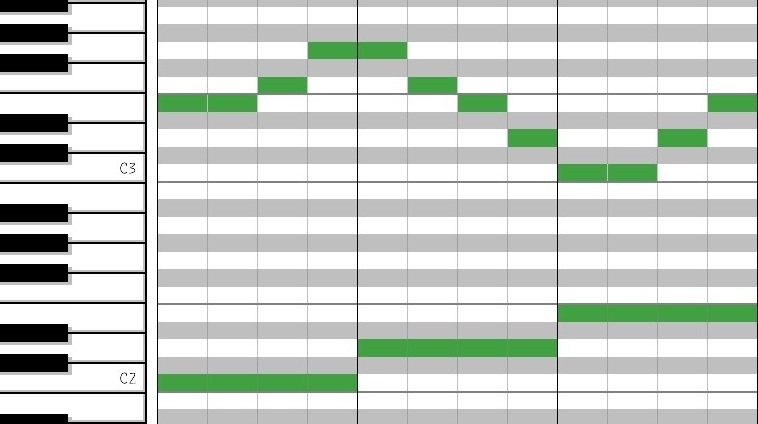
\includegraphics[width=\columnwidth]{imgs/background/piano_roll.jpg}
 \caption{Example of music represented in a piano roll format.}
 \label{fig:piano_roll}
\end{figure}

% Using a piano roll representation with LMs also requires creating a
% vocabulary of symbols to represent notes and their attributes
% (duration and velocity). However, the sequence of symbols is defined
% by the time steps in the piano roll, instead of the stream of events
% in the MIDI representation.

The MIDI representation can be mapped to a piano roll by sampling time steps with a given frequency (e.g. every eighth note). Because of this property, most datasets of symbolic music organize pieces in a collection of MIDI files. For example, the \textit{MAESTRO} dataset \cite{hawthorne2018enabling} is composed of about 200 hours of virtuosic piano performances of classical music pieces captured from the International Piano-e-Competition \cite{yamahaEPiano} in MIDI format aligned with audio waveforms. The \textit{Lakh} \cite{raffel2016learning} dataset is a collection of 176,581 unique MIDI files from various music genres (mostly pop music) scraped from publicly available sources on the internet, where 45,129 of them have been matched and aligned to entries in the \textit{Million Song Dataset} \cite{bertin2011million}. \textit{Piano midi.de} is a dataset of classical piano pieces from a wide variety of composers recorded in MIDI with a digital piano. JSB Chorales \cite{boulanger2012modeling} contains the entire corpus of 382 four-part harmonized chorales by J. S. Bach.

MIDI and piano roll are the most common formats used to represent symbolic music. However, there are also other formats that have been used in the AMC literature. For example, the ABC notation \cite{walshaw1993abc2mtex} is a text-based music notation system popular for transcribing,
publishing and sharing folk music. MusicXML \cite{good2001musicxml} is a markup language that has been designed to facilitate the sharing, exchange, and storage of scores by musical software systems.

To use any of these symbolic music representations with LMs, one has to define a vocabulary that encodes music data into music symbols. These symbols will be used to create sequences that represent music pieces. For example, in a MIDI representation, one has to map the note events into tokens and use the delta-time information from the \textit{track chunks} to define the order of symbols that will form the music pieces. In a piano roll representation, one has to map the vertical axis (pitch) into tokens and process the piano roll grid either horizontally or vertically to define the order of the tokens. To be processed by NNs, each symbol in the vocabulary has to be mapped into a vector. Traditionally, these symbols are mapped using \textit{one-hot} encoding, where each symbol is given an index $i$ and is represented by a vector $v = [v_1, v_2, \cdots, v_n]$ where only $v_i = 1$ and all the other dimensions $v_{j \neq i} = 0$. In the one-hot encoding, $n$ is the number os symbols in the vocabulary.

\section{Neural Networks}

% With a dataset of music represented in a symbolic format (MIDI, piano roll, etc.),
% one can train a ML model to learn a LM that can generate music.
% In early examples, LMs were typically implement with Markov chains and
% recently LMs are more commonly modeled with artificial neural networks.
Artificial Neural Networks, or simply Neural Networks (NNs), interconnect a number of simple processing units called \textit{neurons} to learn a function from training examples. These neurons are typically organized into layers. Neurons might be connected to several other neurons in the layer before it, from which it receives data, and several neurons in the layer after it, to which it sends data. NNs can be defined with different \textit{architectures}, i.e. with a different number of layers (\textit{depth}) and different layouts of neuron connections. The first layer of the network is called the \textit{input layer}, and the last one is called the \textit{output layer}. All the intermediate layers are called \textit{hidden layers}. Each neuron in the hidden or output layers takes as input a vector $x = [x_1, x_2, \cdots, x_n]$ of incoming connections from the previous layer and assigns a weight vector $w = [w_0, w_1, \cdots, w_n]$ to these connections. In its most basic form, the neuron first applies a linear transformation $z = w \dot x + b$ to the inputs $x$, where $b$ is an extra weight called \textit{bias} that is not tied to any neuron of the previous layer. The neuron then uses a nonlinear function called \textit{activation function} $f$ to map the linearly transformed inputs $z$ into an output $\hat{y}$.
Figure \ref{fig:nn} shows a three-layer\footnote{Typically, the input layer is not considered when counting the depth of the NN.} NN called \textit{feedforward} network or \textit{multilayer perceptron} (MLP),
with the computation performed by each layer highlighted besides them. The bias terms have been removed for clarity.

\begin{figure}[!h]
\centering
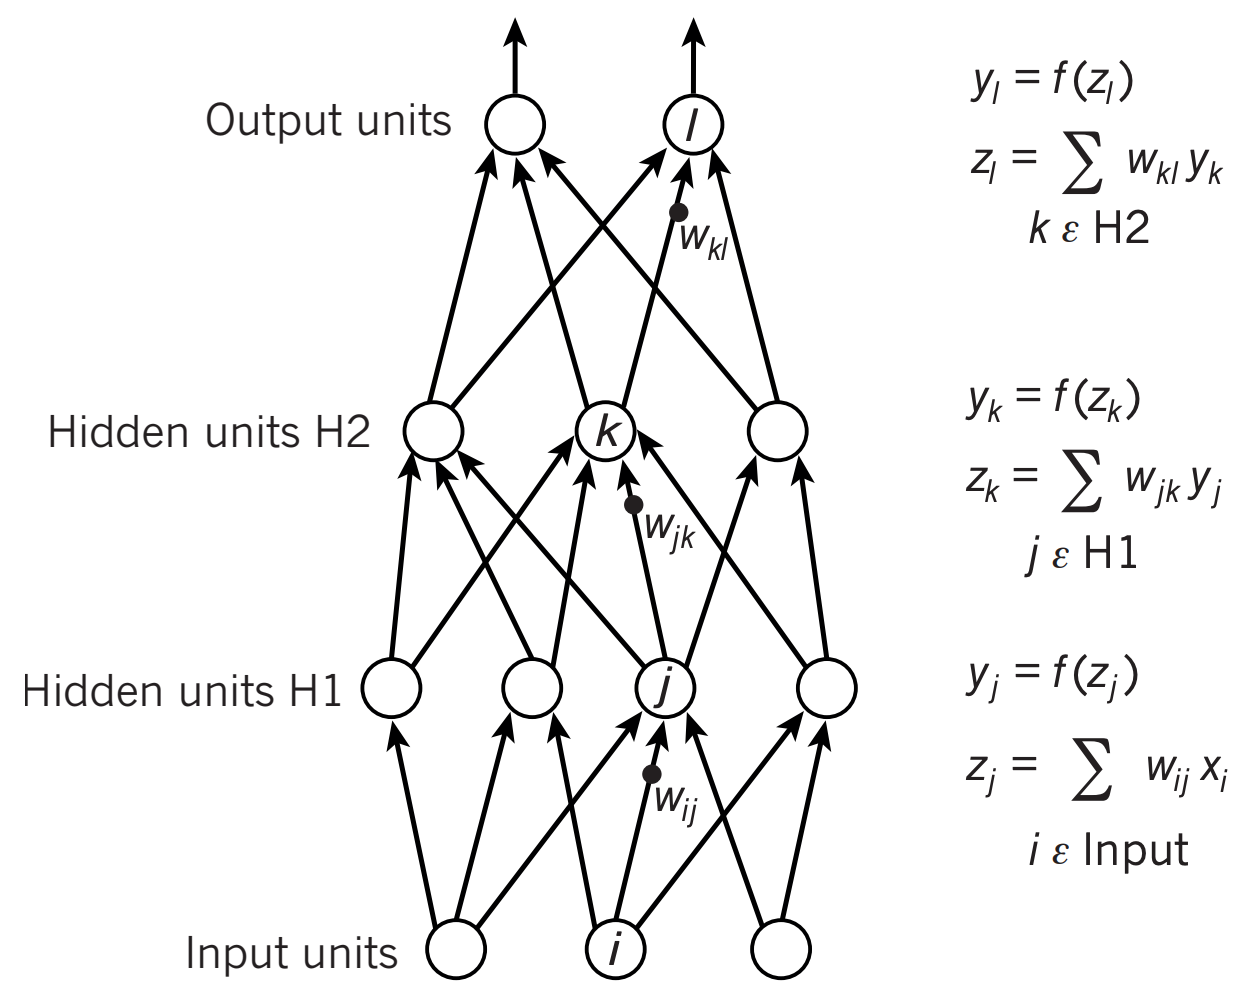
\includegraphics[width=0.7\columnwidth]{imgs/background/ann.png}
\caption{Diagram of a feedforward neural network \cite{lecun2015deep}.}
\label{fig:nn}
\end{figure}

The number of neurons per layer, i.e. the \textit{layer size}, and the layers' activation functions depend on the task that the NN is learning. In traditional supervised problems, the input layer size is defined by how the input examples are represented and the output layer size by the number of classes in the problem. For example, consider a handwritten digits classification problem in which each handwritten digit is stored in a 28x28 grayscale image. The goal is to classify the images into one of the ten digits (zero to nine). The input layer size is 784 neurons, one for each pixel in the image. The output layer size is 10 neurons, one for each class. The size of the hidden layers is defined arbitrarily and should be controlled to optimize the performance (e.g. prediction accuracy) of the network.

In \textit{multiclass} problems, such as the handwritten classification, the \textit{softmax} activation function is used in the output layer to create a probability distribution over the classes. Thus, the NN predicts the class with maximum probability. In \textit{binary} problems, the \textit{logistic} activation function is typically used to map the output layer into a single output $0 \leq \hat{y} \leq 1$. The NN predicts $1$ if $\hat{y} > 0.5$ and $0$ otherwise. The activation functions used in the hidden layers are decided arbitrarily as well, and they also affect the performance of the NNs. Three of the most common activation functions used in the hidden layers are: \textit{logistic}, \textit{tanh}, and \textit{ReLu}. Table \ref{tab:activation} formally describes each of these functions.

\begin{table}[h]
    \centering
    % \setlength{\tabcolsep}{4pt}
    \begin{tabular}{lll}
        \textbf{Name} & \textbf{Function} \\
        Logistic (sigmoid) & $\sigma(x) = \frac{1}{1 + e^{-x}}$ \\
        Hyperbolic tangent (tanh) & $tanh(x) = \frac{e^x - e^{-x}}{e^x + e^-x}$ \\
        Rectified linear unit (ReLu) & $relu(x) = max(0, x)$ \\
        Softmax & $softmax(x) = \frac{e^{x_i}}{\sum_{j=1}^{J} e^{x_j}}$ \\
    \end{tabular}
    \caption{A list of common activation functions in the hidden layer.}
    \label{tab:activation}
\end{table}

NNs are typically trained with some variation of the \textit{gradient descent} (GD) algorithm, which optimizes the weights $W^i$ and $b^i$ of all layers $i$ of the network to minimize a given \textit{loss function} $J(W,b)$. The loss function depends on the task being modeled by the NN. However, in supervised learning, one of the most common losses is the \textit{cross-entropy}, which measures the difference between the training data distribution and the distribution modeled by the NN. Equation \ref{eq:cross_entropy} formally defines the cross-entropy loss for a single example, where $y_c$ is the target label for the class $c$, $\hat{y}_c$ is the output predicted by the $NN_{W^i,b^i}$ with parameters $W$ and $b$ for class $c$, and $C$ is the number of classes in the prediction task.
\begin{equation} \label{eq:cross_entropy}
\begin{split}
    J(W,b) = -\sum_{c=1}^{C} y_clog(\hat{y}_c)
\end{split}
\end{equation}

% In its basic formulation, GD uses the average loss of the entire dataset to update the weights $W^i$ and $b$ of the NN $N_{W,b}$.
As shown in Algorithm \ref{alg:grad_desc}, GD works by iteratively taking steps in the opposite direction of the gradient of the loss function with respect to all weights. For a given number of iterations called \textit{epochs}, GD (line \ref{line:grad}) computes the gradient vector of the loss function $J(W,b)$ for the entire training dataset and (line \ref{line:update}) updates the parameters $W^i$ and $b^i$ in the opposite direction of the gradient. The \textit{learning rate} $\alpha$ is a parameter that controls the size of the training step. Computing the gradient vector (line \ref{line:grad}) requires calculating the partial derivatives of the loss function with respect to all the weights in the NN. This calculation is typically performed by an algorithm called \textit{backpropagation}, which uses the chain rule to compute the gradient one layer at a time, iterating backwards from the output layer to avoid redundant calculations of intermediate terms in the chain rule.

\begin{algorithm}[t]
\caption{Gradient Descent}
\label{alg:grad_desc}
\begin{algorithmic}[1]
\REQUIRE Dataset $(X, Y)$, a loss function $J(W,b)$, a NN $N_{W^i,b^i}$ with
parameters $W^i$ and $b^i$, the number of epochs $e$ and the learning rate $\alpha$.
\ENSURE Updated parameters $W^i$ and $b^i$ of all layers $i$.
\FOR{$i \gets 1$ \TO $e$ }
       \STATE $\partial W^i \gets \frac{\partial J}{\partial W^i}$, $\partial b^i \gets \frac{\partial J}{\partial b^i}$ \label{line:grad}
       \STATE $W^i \gets W^i - \alpha \, \partial W^i$, $b^i \gets b^i - \alpha \, \partial b^i$ \label{line:update}
\ENDFOR
\end{algorithmic}
\end{algorithm}

Calculating the gradients for the whole dataset to perform just one update can be very slow or intractable for datasets that do not fit in memory. \textit{Stochastic Gradient Descent} (SGD) is a variation of GD that solves this problem by splitting the training data into sets called \textit{batches} of size $N$ and performing a parameter update for each one of them.  Although SGD supports training with very large datasets, it introduces convergence issues due to the variance in the frequent updates that cause the value of the loss function to fluctuate. \textit{Adaptive Moment Estimation} (Adam) is a recent variation of SGD that mitigates this problem by having a learning rate per per-parameter and separately adapting them during training \cite{kingma2014adam}. In practice, most practitioners use the Adam optimizer, given that successfull NNs typically require large datasets that do not fit in memory\footnote{The term \textit{big data} is typically used to refer to these very large datasets.}.

\subsection{Recurrent Neural Networks}
\label{sec:rnns}

\textit{Recurrent Neural Networks} (RNNs) are an important architecture for AMC because they were specifically designed to model sequential data. RNNs process sequences $x = [x_1, x_2, \cdots, x_t]$ step-by-step by keeping an internal state $h_t$ that is updated every step. Each element $x_i$ is a vector representing a token (e.g. words in English or pitch classes in western music) traditionally encoded as a one-hot vector. Figure \ref{fig:rnn} shows an abstract diagram of an RNN.

\begin{figure}[!h]
\centering
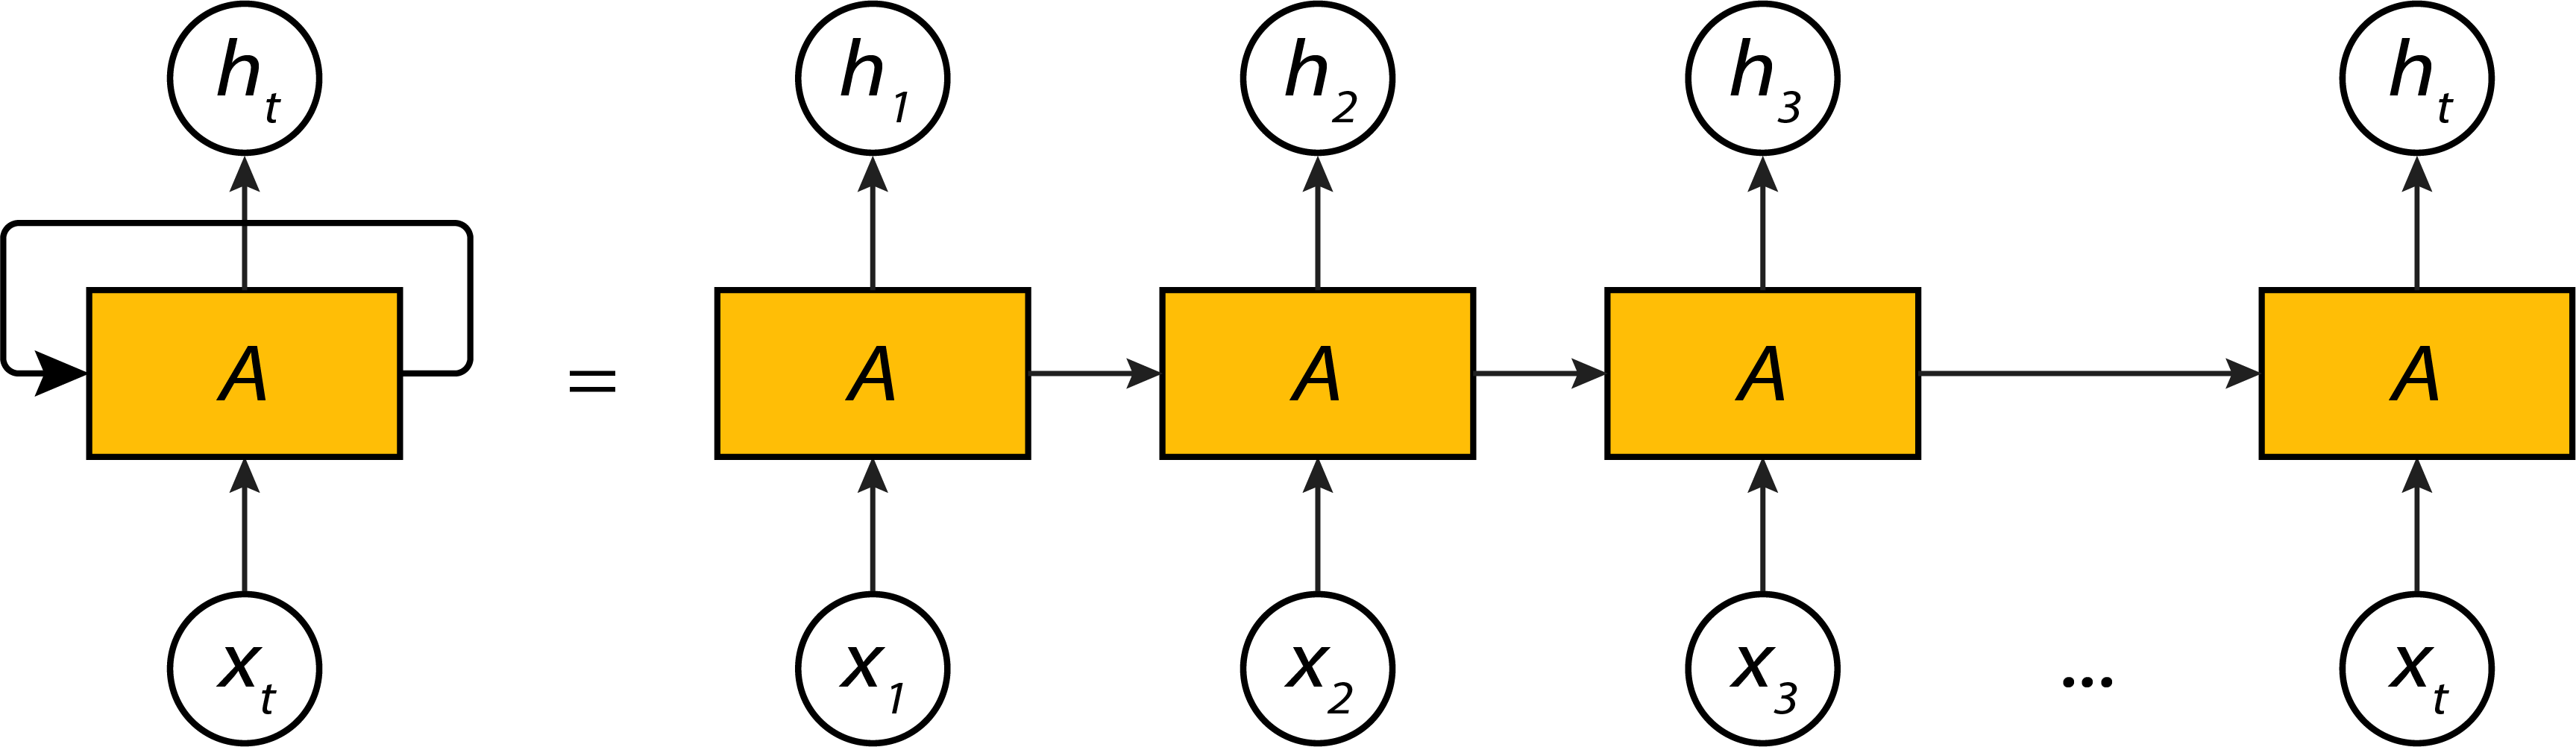
\includegraphics[width=0.9\columnwidth]{imgs/background/rnn.png}
\caption{Diagram of a RNN \cite{olah2015understanding}.}
\label{fig:rnn}
\end{figure}

On the left-hand side, the RNN is shown with an input layer that passes a symbol $x_t$ to a stack of hidden layers $A$ that updates $h_t$. A loop in the hidden layers allows information to be passed from one step of the network to the next. The right-hand side shows an unrolled version of the same RNN. The output layer of the network is omitted from the diagram because RNNs can produce multiple outputs, one per time step or one single output at the very last time step. This configuration depends on the problem. However, the output layer maps a current hidden state $h_t$ to an output vector $y$.

Two of the most simple types of RNNs are the \textit{Elman} and \textit{Jordan} networks. They are RNNs with three layers: an input layer, a single hidden layer, and an output layer. In these networks, an output $y_t$ is produced for each time step $t$. Equation \ref{eq:elman} and Equation \ref{eq:jordan} formally describe these networks, respectively, where $W_{xh}$, $W_{hh}$ and $W_{hy}$ are weight matrices and $\sigma$ are activation functions. The matrices $W_{xh}$, $W_{hh}$ represent the weights of the hidden layer, and the matrix $W_{hy}$ represent the weights of the output layer. The weights $W_{hh}$ are called context units.
\begin{align}
\begin{split}
    h_t &= \sigma(W_{xh}x_t + W_{hh}h_{t-1}) \\
    y_t &= W_{hy}h_t
\end{split}
\label{eq:elman}
\end{align}
\begin{align}
\begin{split}
    h_t &= \sigma(W_{xh}x_t + W_{hh}y_{t-1}) \\
    y_t &= W_{hy}h_t
\end{split}
\label{eq:jordan}
\end{align}

These two networks are very similar. The main difference is that the context units are fed from the output layer instead of the hidden layer. Todd \cite{todd1989connectionist} presented one of the first applications of NNs for music composition: a \textit{Jordan} network designed to generate melodies (monophonic). The input of this network is a melody encoded as a sequence of pitch classes (e.g. \textit{CDEGFEDF}), and the output is a single pitch. This network was trained to reconstruct given example melodies. Each melody contributed to $t$ training steps, where $t$ is the size (number of pitches) of the melody. At every training step $t$, the current example melody is given as input, and the network error is calculated by comparing the network output $y_t$ with the respective pitch $x_t$ of the input melody. After training, one could give new melodies as input to the network, which would create new melodies interpolating between the ones used during the training phase. Duff \cite{duff1989backpropagation} published another early example that is similar to the work of Todd \cite{todd1989connectionist}, but Duff encoded each melody as a sequence of note intervals\footnote{The distance in pitch between two notes.} instead of pitch classes.

One of the major problems of RNNs consists of modeling long-term dependencies between symbols in a sequence. Modeling long-term dependency consists of creating an RNN capable of considering previous symbols that are distant from the one that is being predicted. In practice, simple RNNs are unable to connect the information between symbols that are very far from each other \cite{bengio1994}. In music, modeling long-term dependencies is critical to generate long complete pieces with coherent form.

\subsection{Long Short-Term Memory Networks}
\label{sec:lstm}
% LSTM and GRU

Long Short-Term Memory (LSTM) network \cite{hochreiter1997long} is a special type of RNN explicitly designed to solve the problem of simple RNNs with long-term dependencies. As shown in Figure \ref{fig:rnn}, RNNs have the form of a chain of repeating stacks of layers $A$. LSTMs follow the same structure, but the repeating module performs different computations. Figure \ref{fig:lstm} shows a diagram of a LSTM. A single LSTM module $t$ is composed of an extra state $C_t$ called \textit{cell state}, which is responsible for carrying information through the entire LSTM network. The float of information in the cell state is controlled by four \textit{gates}: an input gate $i_t$, an output gate $o_t$ and a forget gate $f_t$. These gates facilitate the cell to remember or forget information for an arbitrary amount of time.

\begin{figure}[!h]
\centering
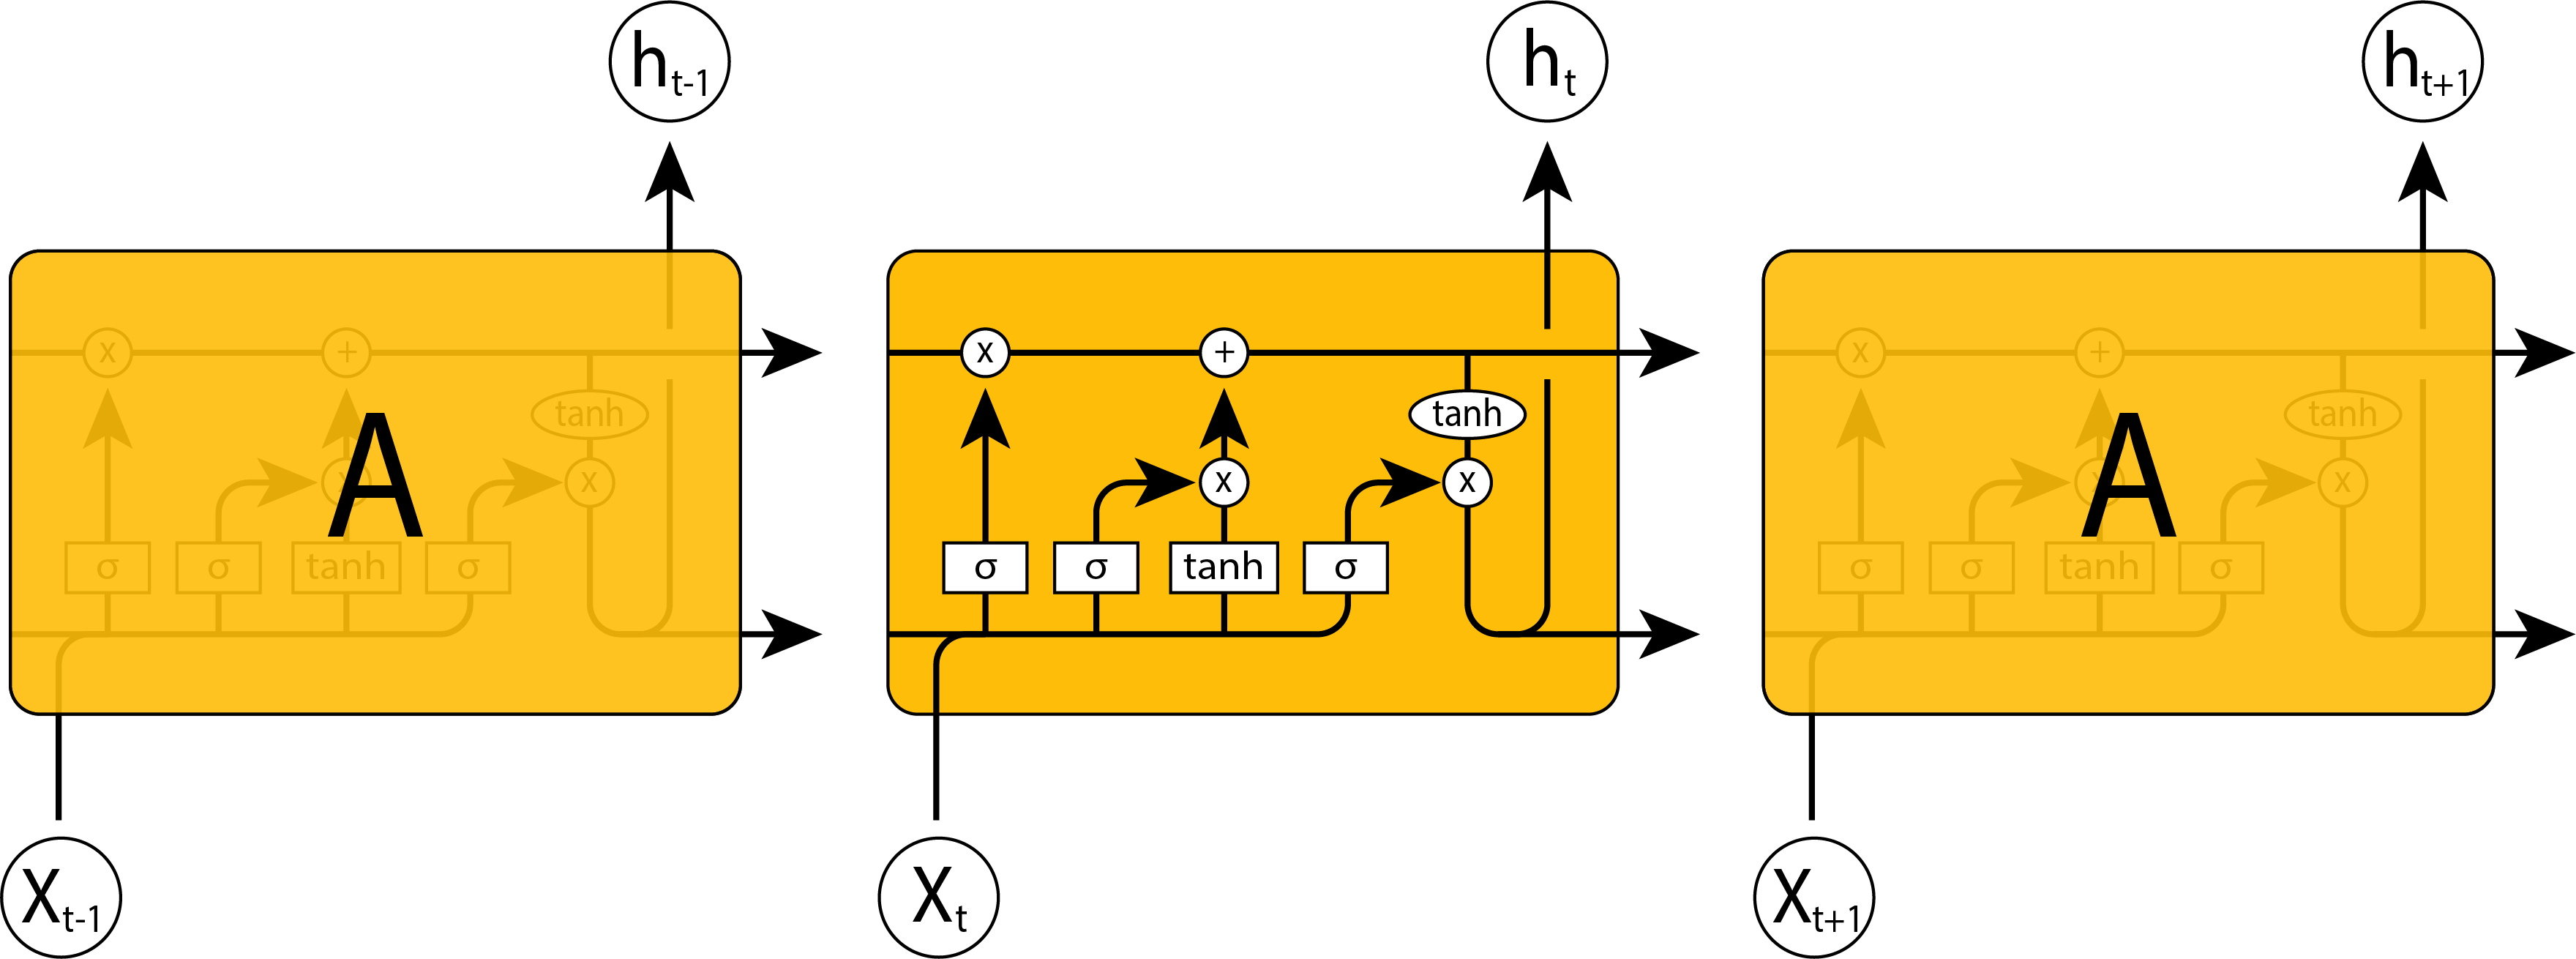
\includegraphics[width=0.9\columnwidth]{imgs/background/lstm.png}
\caption{Diagram of a LSTM \cite{olah2015understanding}.}
\label{fig:lstm}
\end{figure}

Equation \ref{eq:lstm} formally defines the computation performed in each LSTM module, where $W_f$, $W_i$, $W_c$, and $W_o$ are weight matrices, $[h_{t-1}, x_t]$ is the the hidden state vector $h_{t-1}$ concatenated with the input vector $x_t$, and $\tilde{C}_t$ is the candidate vector to added to the cell state.
\begin{equation} \label{eq:lstm}
\begin{split}
    f_t &= \sigma(W_f[h_{t-1}, x_t]) \\
    i_t &= \sigma(W_i[h_{t-1}, x_t]) \\
    \tilde{C}_t &= tanh(W_c[h_{t-1},x_t]) \\
    C_t &= f_t * C_{t-1} + i_t * \tilde{C}_t \\
    o_t &= \sigma(W_o[h_{t-1}, x_t]) \\
    h_t &= o_t * tanh(C_t)
\end{split}
\end{equation}

Each gate $i_t$, $o_t$, and $f_t$ have the exact same equation, just with different weight matrices ($W_i$, $W_o$ and $W_f$, respectively). The cell state $C_t$ combines the input and forget gates to control the amount of information that will be included from the input versus the amount of information that will be forgotten from the current cell state, respectively. The output gate controls the parts of the cell state that will be included in the final hidden state $h_t$. Modern RNNs (including LSTMs) typically have an extra hidden layer that is added before any other hidden layer to transform the one-hot input vectors $x_t$ into \textit{embeddings}. In NLP, a word \textit{embedding} is a learned representation for text where words that have the same meaning have a similar representation. The \textit{embedding} layer learns a dense vector representation of arbitrary dimension from the sparse one-hot representation of the symbols in the vocabulary.

% TODO: Add figure with embedding example
% TODO: bidirectional LSTMs

Early RNNs were not necessarily trained as LMs (see Section \ref{sec:rnns}), but most modern LSTMs compose music as an LM. To learn an LM from an LSTM, one has to map the output at each time step $\hat{y_t}$ to a probability distribution over the symbols in the defined music vocabulary. This is normally done with a \textit{softmax} activation function in the output layer. The LSTM is then trained with mini-batch gradient descent to predict the next symbol $y_{t_1}$ given the current symbol $y_t$ from music pieces given as training data. Many recent deep learning approaches used LSTMs to model music generation with LMs \cite{briot2017deep}. For example, Lyu et. al. \cite{lyu2015modelling} combined an LSTM with another type of neural network called Restricted Boltzman Machine (RBM) to generate polyphonic music with different musical styles. They experimented with both the Musedata and the JSB Chorales \cite{boulanger2012modeling}. The pieces were encoded as a sequence of pitch numbers temporally aligned on an integer fraction of a quarter note. This encoding system only considered pitch and duration and hence did not considered dynamics information (e.g. note velocity).

BachBot \cite{liang2017automatic} uses a deep LSTM to generate polyphonic in the style of Bach’s chorales. BachBot was trained with the JSB Chorales dataset, where each chorale was encoded with a sequence of sixteenth-note frames. Each frame consisted of four tuples (Soprano, Alto, Tenor, and Bass), and each tuple in the form (\textit{pitch}, \textit{tie}), where \textit{pitch} represents a MIDI pitch and \textit{tie} is a boolean value that distinguishes whether a note is tied with a note at the same pitch from the previous frame or is articulated at the current time step. This encoding system also did not consider dynamics information. Oore et al. \cite{oore2017learning} propose one of the first methods that can generate music with dynamics. They trained an LSTM with a new representation that supports tempo and velocity events from MIDI files. This model was trained on the MAESTRO \cite{hawthorne2018enabling}. With this new representation and dataset, Oore et al. \cite{oore2017learning} generated more human-like performances when compared to previous models.

\subsection{Transformers}

\textit{Transformer} \cite{vaswani2017attention} is a modern architecture for sequence modeling based on \textit{attention} mechanisms, as opposed to recurrent layers. In NLP, an attention mechanism is a part of a neural architecture that enables highlighting relevant words of the input sequence dynamically. Instead of keeping an internal hidden state that is updated at each time step like RNNs, transformers process entire sequences associating an \textit{attention} score to each token that determines how much that token contributes to the output of the network. Because transformers process tokens in parallel, they can take advantage of the parallel computing offered by GPUs, and hence transformers can be trained considerably faster than LSTMs \cite{vaswani2017attention}. One drawback of the transformers is that they can only process sentences with a fixed size instead of LSTMs that can process sentences of any size.

Transformers were originally designed in the context of \textit{machine translation}, an NLP task that consists of translating a sequence from one language (e.g. English) to another (French). Machine translation is a \textit{sequence-to-sequence} problem, where a sequence input $x$ has to mapped into an output sequence $y$. NNs designed for machine translation normally have a \textit{encoder-decoder} structure. The first part of the network, called the \textit{encoder}, takes a sequence as input $x$ and outputs a vector representation $e$ (called \textit{encodings}) of the input $x$. The second part, called \textit{decoder}, takes the encodings $e$ as input and outputs a sequence $y$. As shown in Figure \ref{fig:transformer}, the transformer has an encoder-decoder structure (the encoder is showed on the left side and the decoder on the right side). The transformer takes as input a sentence typically encoded as one-hot vectors and transforms it into two sequences: a sequence of \textit{word embeddings} and a sequence of \textit{positional embeddings}. The former is a dense vector representation of words learned from the sparse one-hot input. The latter is also a dense vector representation but learned from the position (indices) of the words in the input sentence. The transformer adds the input embeddings and positional encodings together and passes the result through the encoder, followed by the decoder.

% TODO: Add figure with input + positional embedding example

\begin{figure}[!h]
 \centering
 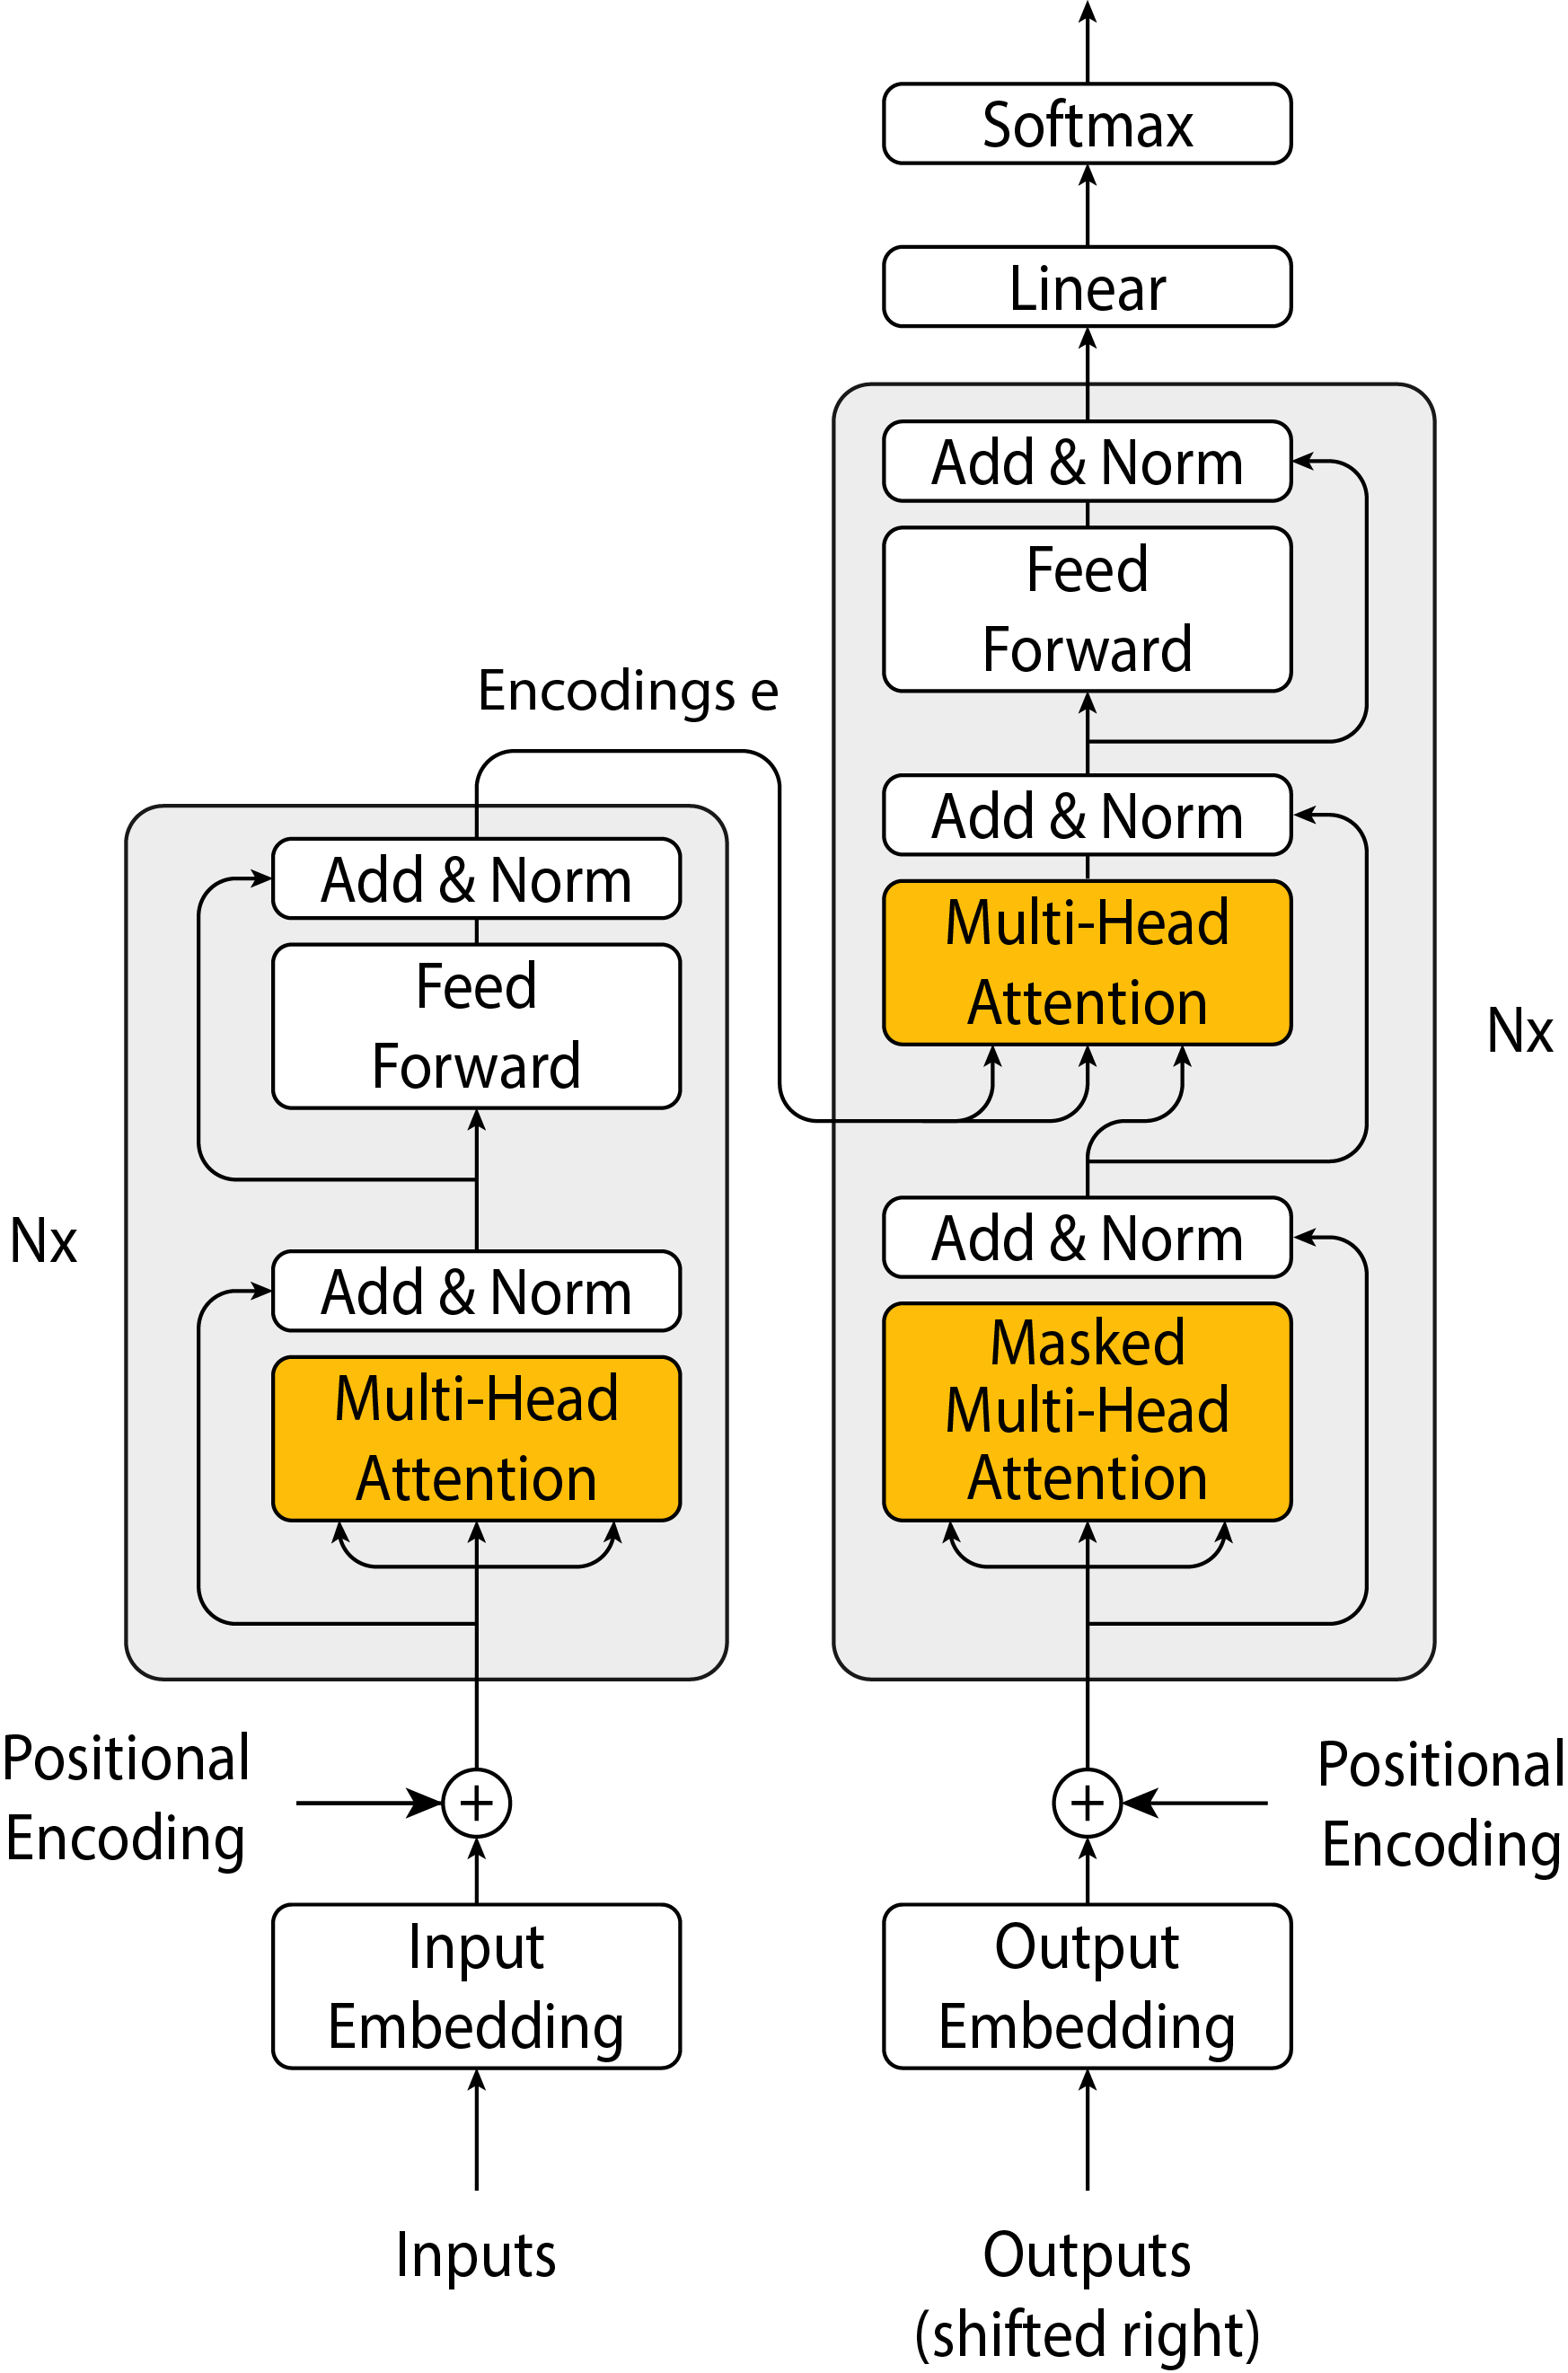
\includegraphics[width=0.5\columnwidth]{imgs/background/transformer.png}
 \caption{Diagram of a Transformer \cite{vaswani2017attention}.}
 \label{fig:transformer}
\end{figure}

The encoder converts the (input + position) embeddings $e$ into \textit{encodings} with a stack of $n$ identical layers called \textit{transformer blocks}. Each transformer block has two layers: a \textit{multi-head attention layer} and a fully connected \textit{feedforward layer}. A residual connection \cite{he2016deep} is applied around each of the two layers, followed by a layer normalization \cite{ba2016layer}. A residual connection is a connection between non-contiguous layers. A layer normalization is an extra layer that normalizes the activations of the previous layer, i.e. it applies a transformation that maintains the mean activation within each example close to 0 and the activation standard deviation close to 1.

The most important part of the transformer architecture is the \textit{multi-head attention layer}, which computes a score matrix $Z$ from the embeddings $e$, where the scores in $Z$ represent the relationship between different words in the input sentence. For example, consider the sentence ``The animal didn't cross the street because it was too tired.''. In this sentence, the word ``it'' is related to ``animal'', and so when the transformer is processing the word ``it'', self-attention allows it to associate ``animal'' with ``it''. Figure \ref{fig:attn} shows the encoder self-attention distribution for the word ``it'' in this example.

\begin{table}[h]
    \centering
    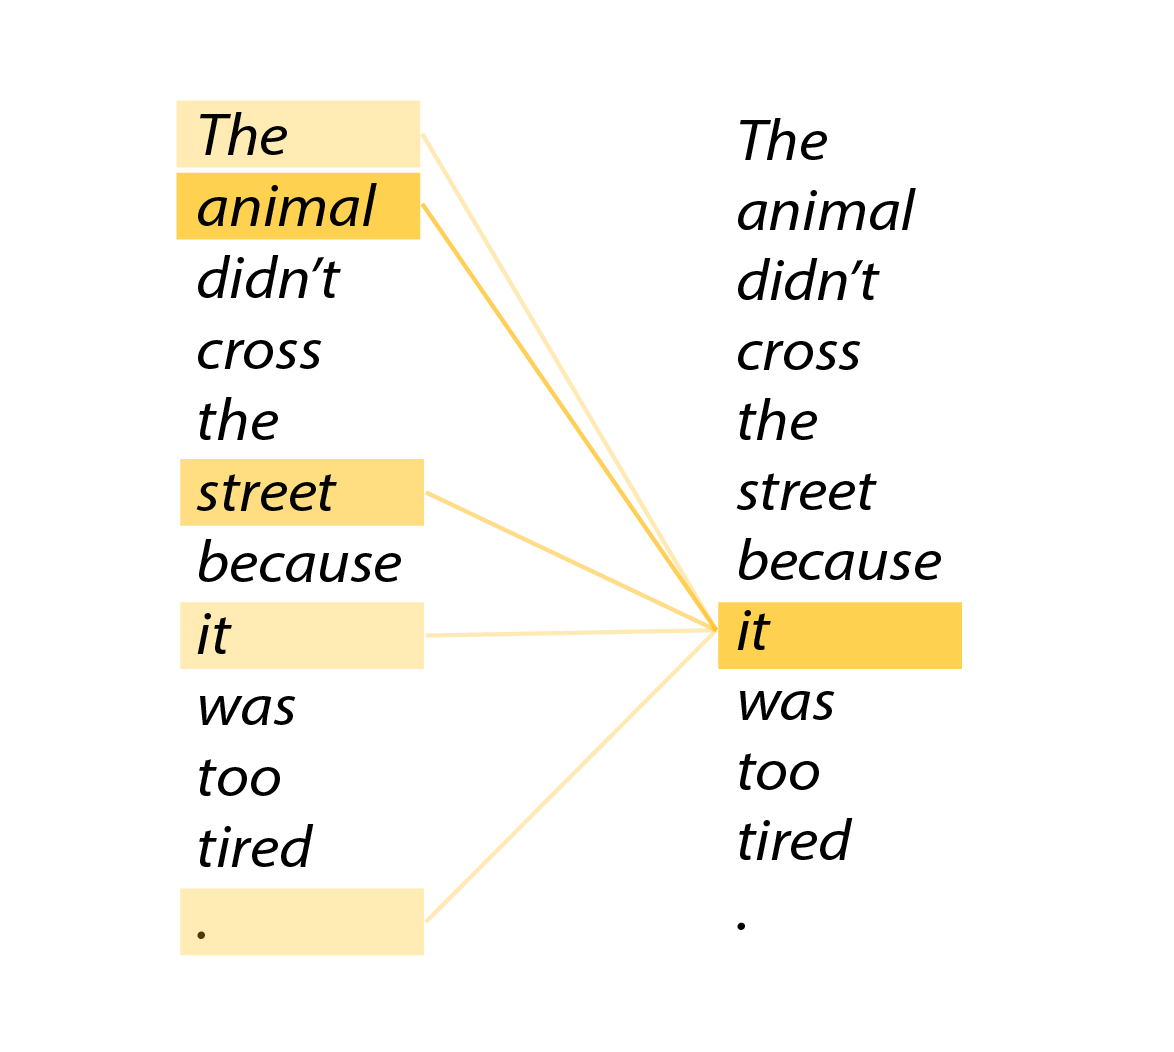
\includegraphics[width=0.5\columnwidth]{imgs/background/attn.png}
    \caption{The encoder self-attention distribution for the word ``it'' in the sentence
    ``The animal didn't cross the street because it was too tired.'' \cite{vaswani2017attention}.}
    \label{fig:attn}
\end{table}

The score matrix $Z$ is computed similarly to a dictionary lookup: it takes a \textit{query} matrix $Q$, a \textit{key} matrix $K$, and a \textit{value} matrix $V$, and outputs a weighted sum of the values that correspond to the keys that are most similar to the query. One of the most common self-attention mechanisms in a transformer neural network is the scaled dot-product attention, which is shown in Equation \ref{eq:attn}. The matrices $Q$, $K$, and $V$ are created by packing the embeddings $e$ of all the words in the input sentence into a matrix $E$, and multiplying it by the weight matrices $W_q$, $W_k$ and $W_v$ that are learned during training.

\begin{equation}\label{eq:attn}
\begin{split}
    Z = Attention(Q, K, V) &= softmax(\frac{QK^T}{\sqrt{d_k}})V \\
    Q &= E * W_q \\
    K &= E * W_k \\
    V &= E * W_v
\end{split}
\end{equation}

The decoder is similar to the encoder, but it has an extra attention layer added before the other two to perform multi-head attention over the target output sentence $y$. This extra layer uses a mask to ensure that the predictions for position $i$ can depend only on the known outputs at positions less than $i$. The output of the decode is a linear layer followed by a softmax activation.

One can take the decoder portion of the transformer to train a LM capable of generating sequences such as text or music similar to a LSTM LM (see Section \ref{sec:lstm}). Equation \ref{eq:transformer} formally defines a decoder-based transformer LM, where $x = [x_1, x_2, \cdots, x_t]$ is the input sequence, $n$ is the number of layers, $W_i$ is input embedding weight matrix, and $W_p$ is the position embedding weight matrix.

\begin{equation}\label{eq:transformer}
\begin{split}
    h_0 &= W_ix + W_p \\
    h_l &= transformer\_block(h_{l-1}) \forall i \in [1,n] \\
    P(u) &= softmax(h_nW_e^T)
\end{split}
\end{equation}

Transformers are currently the state-of-the-art of both natural and music language modeling. Radford et. al. \cite{Radford2018, radford2019language} proposed a series of models called GPT (General Pre-trained Transformer), GPT-2, and GPT-3 that used only the decoder part of the original transformer to create a model of natural language. Radford et. al. showed that besides generating long coherent sequences of text, pre-trained GPT models can be fine-tuned with a simple extra linear layer to perform specific NLP tasks (e.g. commonsense reasoning, question answering, summarization, and others) with state-of-the-art performance. Pre-training consists of training the GPT model as a (unsupervised) LM with a huge general dataset (e.g. Wikipedia). Fine-tuning is performed by adding an extra linear layer to the pre-trained transformer and training this layer with a smaller dataset explicitly created for the task (supervised).

Music Transformer \cite{huang2018music} is one of the first decoder-transformer to generate music. It uses a new relative attention mechanism that improves memory consumption of the original decoder, and hence it can process longer sequences. Music Transformer achieves state-of-the-art performance on the MAESTRO dataset \cite{hawthorne2018enabling}. Donahue et. al. \cite{donahue2019lakhnes} showed that a decoder-transformer could also compose multi-instrument scores by training it with the NES MDB \cite{donahue2018nesmdb} dataset. Donahue et al. improved the performance of their model with a pre-training procedure similar to Radford et al. \cite{Radford2018}. The transformer was first pre-trained with the diverse Lakh dataset (multiple instruments) and then fine-tuned with NES-MDB (four instruments). They manually defined a mapping between the instruments from the two datasets. Pop Music Transformer \cite{huang2020pop} is a transformer model with a specialized music representation to compose pop piano music. It was shown to generate a better rhythmic structure than previous transformer models.

% TODO: Convolutional Neural Networks

\subsection{Variational Autoencoders}

\textit{Variational Autoencoders} (VAEs) \cite{kingma2013auto} are another modern architecture that can be used to generate music. VAEs are different from RNNs and Transformers because they were not specifically designed to model sequences. Instead, they are generative models that can potentially learn to represent any data. VAEs have an architecture similar to a traditional \textit{Autoencoder}, which is an encoder-decoder NN used to learn efficient encodings of unlabeled data (unsupervised learning). Figure \ref{fig:ae} shows a diagram of an autoencoder.

\begin{figure}[!h]
 \centering
 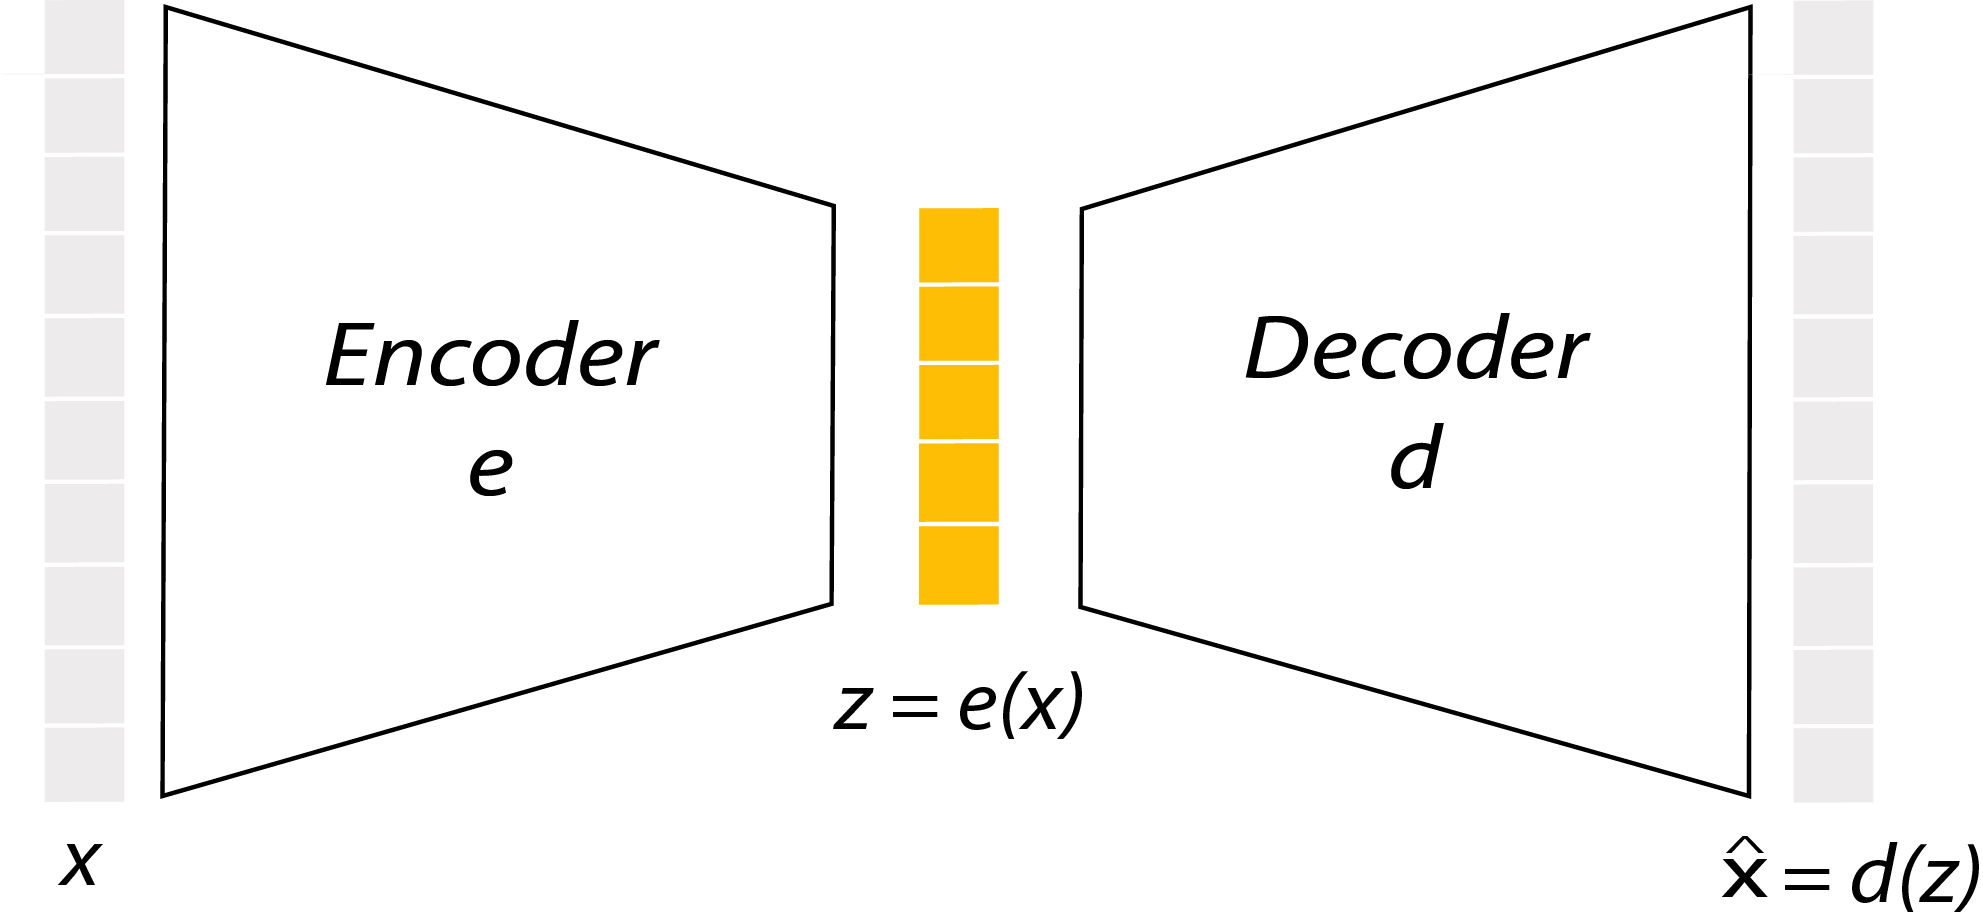
\includegraphics[width=0.8\columnwidth]{imgs/background/autoencoder.png}
 \caption{Diagram of an Autoencoder \cite{rocca2019understanding}.}
 \label{fig:ae}
\end{figure}

An autoencoder builds a latent space of a dataset $X$ with an encoder network $e$ by learning to compress each example $x$ into a vector $z$ and then reproducing $x$ from $z$ with a decoder network $d$. A key component of an autoencoder is the bottleneck introduced by making the vector have fewer dimensions than the input data itself, which forces the model to learn a compression scheme. During training, the autoencoder ideally distills the qualities that are common throughout the dataset. As shown in Figure \ref{fig:ae_sampling}, one can use an autoencoder as a generative model by sampling random vectors from the latent space learned by the encoder and using the trained decoder to build the output from the sampled vector.

\begin{figure}[!h]
 \centering
 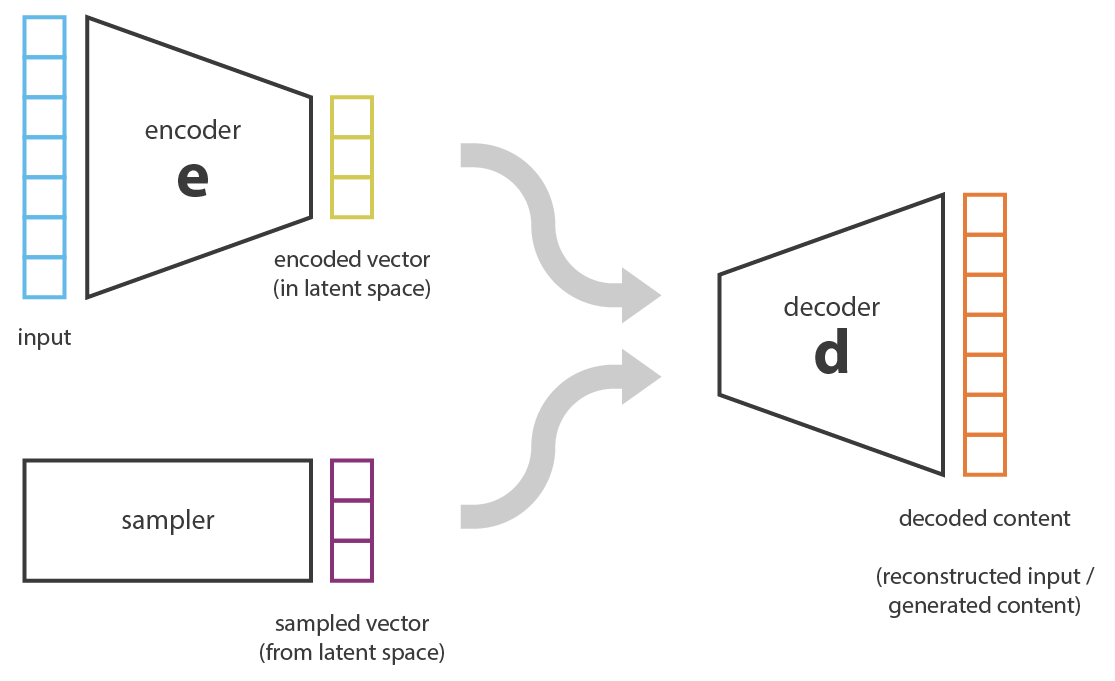
\includegraphics[width=0.8\columnwidth]{imgs/background/ae_sampling.png}
 \caption{Sampling from the latent space built by an Autoencoder \cite{rocca2019understanding}.}
 \label{fig:ae_sampling}
\end{figure}

One limitation of the autoencoder is that it often learns a latent space that is not continuous\footnote{Two close points in the latent space should yield similar outputs when decoded.} nor complete\footnote{Any point sampled from the latent space should yield a ``meaningful'' output when decoded}. This means that if one decodes a random vector sampled from the learned latent space, it might not result in a realistic output. VAEs solve this problem by encoding the dataset $X$ as a probability distribution over the latent space instead of a single vector $z$. Typically, this distribution is assumed to be a multivariate normal distribution $N(\mu_x, \sigma_x)$. Figure \ref{fig:vae} shows a diagram of a VAE. The difference between autoencoders and VAEs is that the encoder of the VAE outputs two vectors $\mu_x$ and $\sigma_x$, instead of a single vector $z$. These two vectors represent the mean and standard deviation of a normal distribution $N$. The decoder samples a vector $z \sim N(\mu_x, \sigma_x)$ from the distribution $N$ and reconstructs the input $x$ from the sampled $z$ using the decoder $d$.

\begin{figure}[!h]
 \centering
 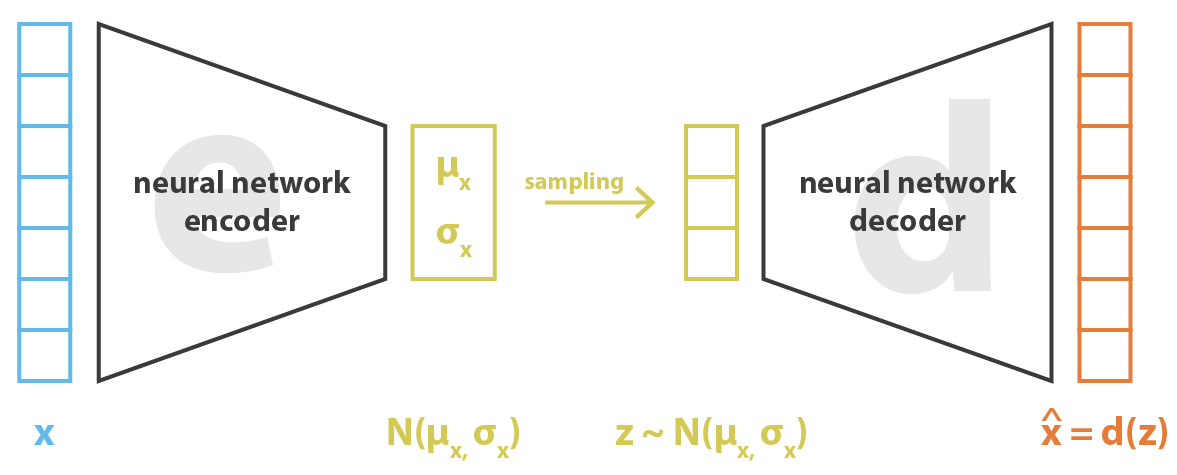
\includegraphics[width=0.8\columnwidth]{imgs/background/vae.png}
 \caption{Diagram of a Variational Autoencoder (VAE) \cite{rocca2019understanding}.}
 \label{fig:vae}
\end{figure}

MusicVAE \cite{Roberts2017} is one of the first examples of VAE applied to music generation. It start by splitting the input sequence $x$ in to $U$ non-overlapping subsequences $y_u$, such that $x = [y_1, y_2, \cdots, y_U]$. The encoder process the segmented input $x$ with a bidirectional LSTM network that outputs two hidden states $\overleftarrow{h_t}$ and $\overrightarrow{h_t}$ that are concatenated to form a final hidden state $h_t$. The final hidden state $h_t$ is fed into two fully connected layers to produce the latent distribution parameters $\mu$ and $\sigma$. The decoder is a novel hierarchical LSTM that takes the latent vector $z \sim N(\mu_x, \sigma_x)$ as input and first produces $U$ embedding vectors $c = [c_1, c_2, \cdots, c_U]$, one for each subsequence $y_u$. An LSTM called the \textit{conductor} produces these embedding vectors, where the hidden state is initialized by passing $z$ through a fully connected layer followed by a \textit{tanh} activation function. Once the conductor has produced the sequence of embedding vectors $c$, each one is individually passed through a shared fully connected layer followed by a tanh activation to produce initial states for a final decoder LSTM. The decoder RNN then autoregressively produces a sequence of distributions over output tokens for each subsequence $y_u$ via a softmax activation in the output layer. At each step of the final LSTM, the current conductor embedding $c_u$ is concatenated with the previous output token to be used as the input.

MIDI-VAE \cite{brunner2018midi} uses a VAE to perform style transfer in polyphonic symbolic music. It works by separating a portion of the latent vector $z$ for style classification $z_s$, and another part $z_t$ to encode the characteristics of the music dataset. During generation, one can change the style $S_i$ of a given input piece $x$ to another style $S_j$ by passing a given input piece through the encoder to get $z$ and swapping the values of dimensions $z_s^i$ and $z_s^j$, and passing the modified latent vector through the decoder. Style labels can be music genres such as Jazz, Pop, and Classic; or composer names such as Bach or Mozart. VirtuosoNet \cite{jeong2019virtuosonet} is a VAE designed to generate piano performances with expressive control of tempo, dynamics, and articulations. The encoder is a hierarchical LSTM such that the input music is encoded on different levels: note, beat, and measure. The decoder renders musical expressions consistently over long-term sections by first predicting the tempo and dynamics in measure level and, based on the result, refining them in note level.

\subsection{Generative Adversarial Networks}

Similar to VAEs, \textit{Generative Adversarial Networks} (GANs) \cite{goodfellow2014generative} are powerful generative models that, in theory, can generate synthetic data in different domains. GANs are composed of two independent NNs: a \textit{generator} and a \textit{discriminator}. In its most basic form, the generator takes random noise as input and then transforms this noise into a fake example. The discriminator is a binary classifier that discriminates examples as \textit{fake} (0) or \textit{real} (1). The generator and the discriminator architectures depend on the data type (e.g. text, images, videos) that is being modeled. For example, Figure \ref{fig:gan} illustrates a GAN for handwritten digit generation. In this case, the random noise is a matrix $M$ representing a grayscale image. A simple way to generate such a matrix is to sample grayscale values between 0 (black) and 1 (white) from a uniform distribution. The generator transforms the random matrix $X$ into a fake handwritten digit normally using convolutional layers. The discriminator combines real and fake images to learn how to separate them between fake and real.

\begin{figure}[!h]
 \centering
 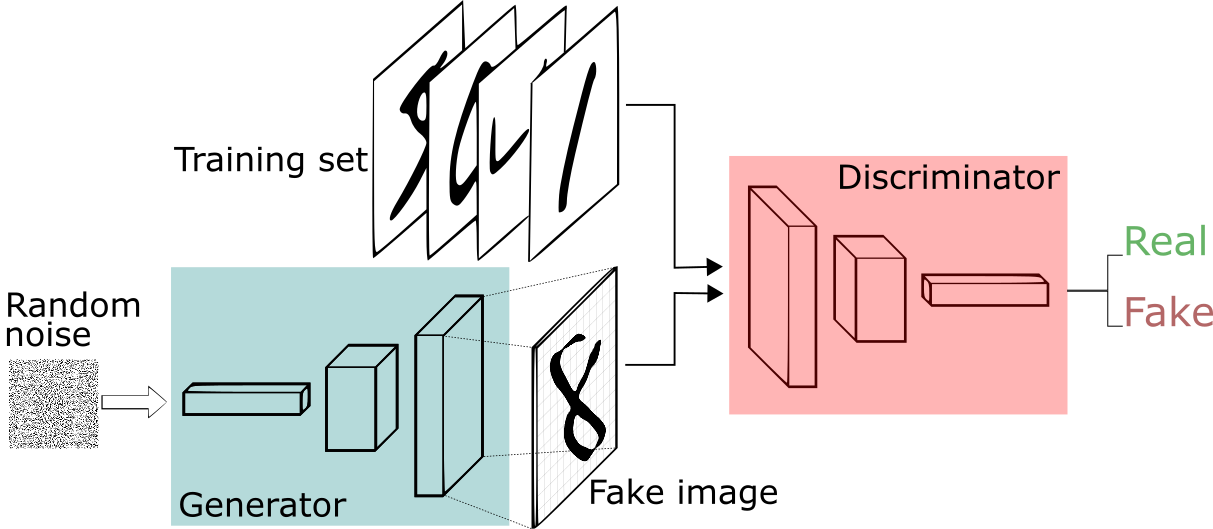
\includegraphics[width=\columnwidth]{imgs/background/gan.png}
 \caption{Diagram of a Generative Adversarial Network (GAN) \cite{silva2018intuitive}.}
 \label{fig:gan}
\end{figure}

Training a GAN consists of training the generator and the discriminator together
iteratively in alternating periods:

\begin{enumerate}
    \item The discriminator trains for one or more epochs.
    The discriminator is trained with a loss function that penalizes the discriminator for misclassifying a real instance as fake or a fake instance as real. The discriminator updates its weights through backpropagation from the discriminator loss through the discriminator network.

    \item The generator trains for one or more epochs.
    The generator is trained with a loss function that penalizes the generator for producing a sample that the discriminator network classifies as fake. In other words, the generator loss is computed via the discriminator. Thus, the generator updates its weights through backpropagation from the discriminator to the generator. It's important to highlight that only the generator weights are updated during generator training.
\end{enumerate}

The original GAN uses a single loss function called \textit{minimax loss} to train both the generator and the discriminator. Minimax loss is derived from the cross-entropy loss between the real and generated distributions. The generator tries to minimize this loss while the discriminator tries to maximize it. Equation \ref{eq:minimax_loss} formally defines the minimax loss, where $D(x)$ is the discriminator's estimate of the probability that real data instance x is real, $E_x$ is the expected value over all real data instances, $G(z)$ is the generator's output when given noise z, $D(G(z))$ is the discriminator's estimate of the probability that a fake instance is real, and $E_z$ is the expected value over all generated fake instances $G(z)$.

\begin{equation} \label{eq:minimax_loss}
    E_x[log(D(x))] + E_z[log(1 - D(G(z)))]
\end{equation}

During training, $G$ learns to generate fake data that resembles the original data, and $D$ learns to distinguish the generator's fake data from real data. The training process aims to have a generator $G$ that produces output that can fool the discriminator $D$. After training, one can generate new data points by sampling from different distribution points learned by $G$. This approach works well to generate continuous data such as images \cite{brock2018large}, but it has limitations in generating categorical data, especially in a sequential form such as text or music. Images can be represented by a continuous matrix $M$ and so applying transformations (e.g. $M' = M + 0.05$) to $M$ still results in defined images $M'$ that can be classified as real or fake by a discriminator. In sequential domains such as text and music, tokens are encoded using embedding vectors. Applying transformation to an embedding vector does not necessarily generate a valid token. For example, assume that the word ``university'' is represented by the vector $v = [0.44, 0.37, -0.28]$. If one applies the transformation $v' = v + 0.05$ to the original $v$, the new vector $v'$ not necessarily represent some word in the vocabulary. Therefore, updating the weights of $G$ with the gradients of the minimax loss might lead $G$ to generate invalid data. Another problem is that the discriminator can only provide feedback on entire sequences.

% TODO: Better summarize and correlate the different approaches
Different approaches have been proposed to solve these problems in the domain of symbolic music generation. For example, C-RNN-GAN \cite{yang2017midinet} generated polyphonic music as a series of note events by introducing some ordering of notes and using RNNs in both the generator and the discriminator. SeqGAN \cite{yu2017seqgan} combined GANs and reinforcement learning to generate monophonic music with an RNN generator and a CNN discriminator. MidiNet \cite{yang2017midinet} used GANs with conditional CNNs as both generator and the discriminator to generate melodies that follow a chord sequence given a priori, either from scratch or conditioned on the melody of previous bars. MuseGAN \cite{dong2018musegan} generates polyphonic music by encoding multi-track measures as a piano roll and also modeling both the generator and the discriminator as CNNs. Muhamed et al. \cite{muhamed2021symbolic} modeled both generator and the discriminator as transformers and used the Gumbel-Softmax trick \cite{jang2016categorical} to address the gradient problem of categorical generators.

\section{Decoding}

As discussed in the previous section, most neural generative models for AMC are based on architectures specially designed to model sequences: RNNs, LSTMs, and Transformers. Formally, these sequential models use a softmax activation function in the output layer to create a LM $L = P(x_t|x_1, \cdots, x_{t-2}, x_{t-1})$, where $\{x_1, \cdots, x_{t-2}, x_{t-1}\}$ is an input sequence and $x_t$ is the next token in that sequence. Typically, an \textit{autoregressive} strategy is used to generate music with $L$, i.e. to \textit{decode} the softmax output into a sequence of music tokens. Namely, one starts with a prior sequence of tokens $x = [x_1, x_2, \cdots, x_{t 1}]$, which are fed into $L$ to generate $L(x) = x_{t}$. Next, $x_{t}$ is concatenated with $x$ and the process repeats until a special end of-piece symbol is found or a given number of symbols are generated. As defined in Equation \ref{eq:autoregressive}, autoregressive generation assumes that the probability distribution of a sequence of tokens can be decomposed into the product of conditional next token distributions.

\begin{equation} \label{eq:autoregressive}
    P(x_t|x_1, \cdots, x_{t-2}, x_{t-1}) = \prod_{t=1}^{T} P(x_t|x_{1:t-1})
\end{equation}

Currently, most prominent \textit{autoregressive} strategies for music (and text) decoding are based either on \textit{sampling} or \textit{searching}. While sampling is well suited for creative tasks such as music composition, searching fits better generative problems where specific solutions are expected, such as machine translation.

\subsection{Top-k Sampling}

In its most basic form, sampling consists of randomly picking the next token according to the conditional probability distribution given by the LM: $x_t \sim P(x_t|x_{1:t-1})$. Figure \ref{fig:topk} shows and example where the prior is the sequence $x = [\textit{The}]$. In the first step, the word \textit{car} is sampled from the condition probability distribution $P(x_1 | \textit{The})$ and, in the second step, the word \textit{drives} is sampled from $P(x_2 | \textit{The}, \textit{car})$.

\begin{figure}[!h]
 \centering
 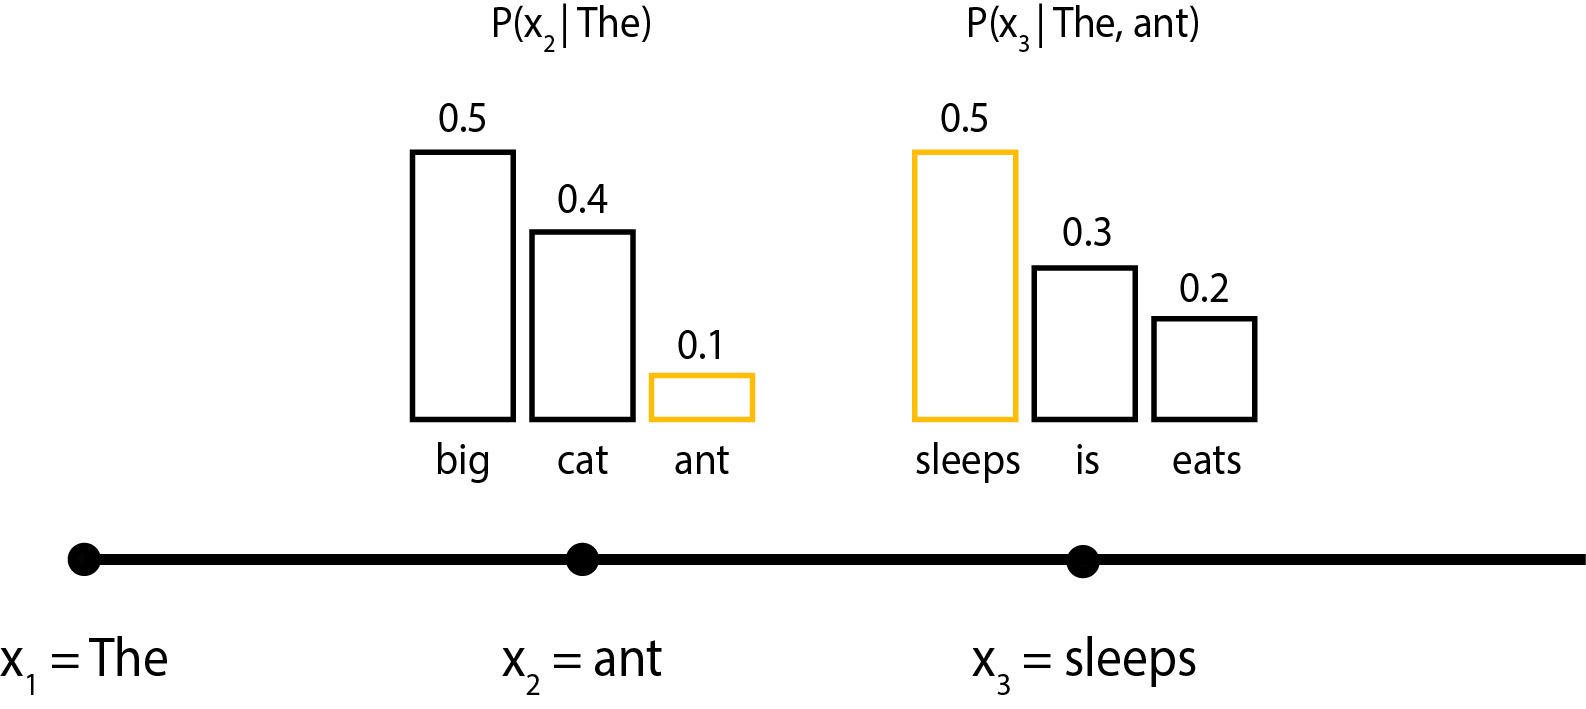
\includegraphics[width=0.9\columnwidth]{imgs/background/sampling.png}
 \caption{Example of sampling for text generation with prior $x = [\textit{The}]$ \cite{platen2020}.}
 \label{fig:topk}
\end{figure}

A simple trick called \textit{temperature} can be applied to control the confidence of the LM. It consists of dividing the result of the model output layer before the softmax activation by a parameter $t > 0$. Lower temperatures $t < 1$ makes the model increasingly confident in its top choices, while $t > 1$ decreases confidence. Figure \ref{fig:temp} shows the previous sampling example with temperature $t = 0.7$. The conditional probability $P(x_1 | \textit{The})$ of the first step becomes more confident, leaving almost no chance for the word \textit{car} to be selected. Thus, the first sampled word is \textit{nice} followed by the word \textit{house}.

\begin{figure}[!h]
 \centering
 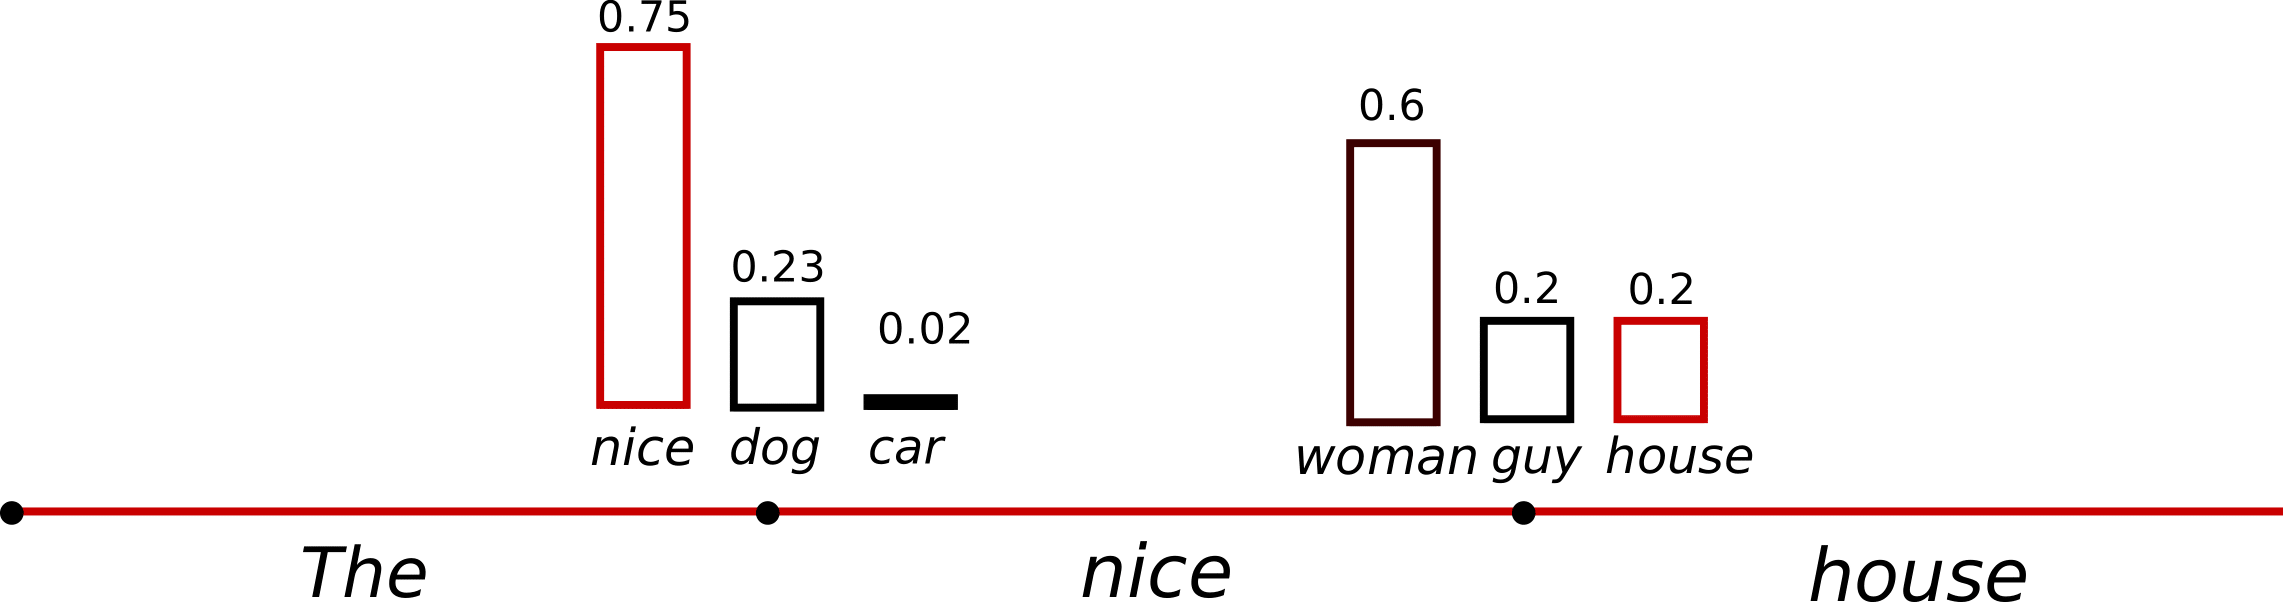
\includegraphics[width=0.9\columnwidth]{imgs/background/temperature.png}
 \caption{Example of sampling for text generation with temperature $t = 0.7$ and
 prior $x = [\textit{The}]$ \cite{platen2020}.}
 \label{fig:temp}
\end{figure}

\textit{Top-k sampling} \cite{fan2018hierarchical} is another way to control the probability distribution of the LM. It consists of using only the $k$ most likely tokens in the distribution, redistributing the probability mass among only those \textit{top-k} words. With this approach, the LM is filtered at each generation step and the token is picked randomly according to the resuling probability distribution. Figure \ref{fig:topk} illustrates a text generation example with top-k sampling where $k=6$.

\begin{figure}[!h]
 \centering
 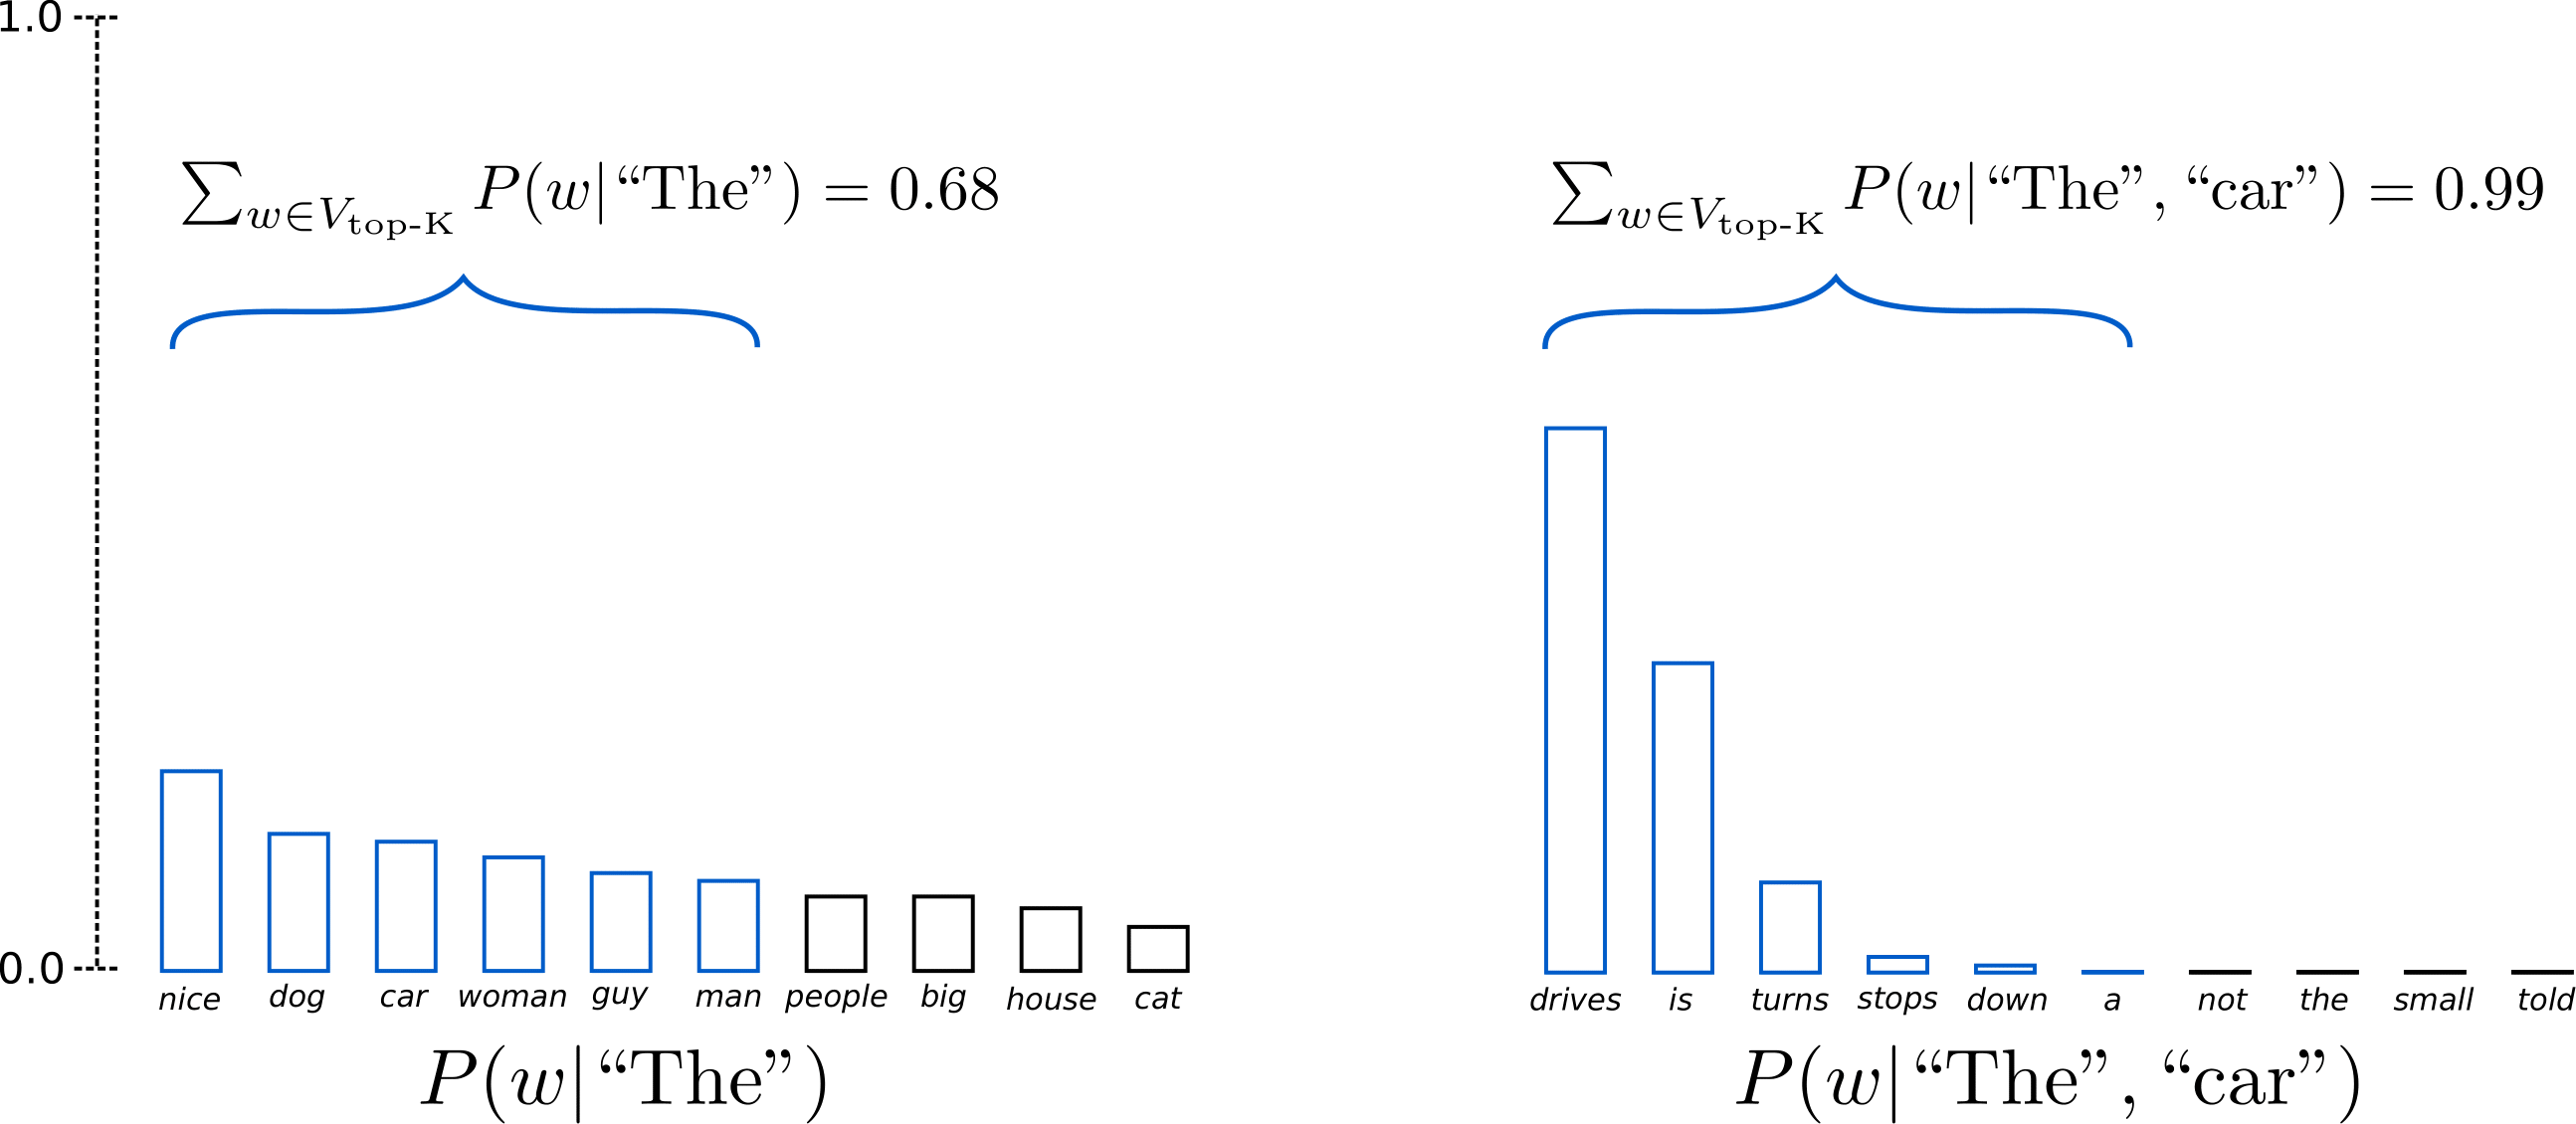
\includegraphics[width=0.9\columnwidth]{imgs/background/topk.png}
 \caption{Example top-k sampling for text generation with $k=6$ and prior $x = [\textit{The}]$ \cite{platen2020}.}
 \label{fig:topk}
\end{figure}

In step $t=1$, the top-k sampling keeps the six words $\{\textit{nice}, \textit{dog}, \textit{car}, \textit{woman}, \textit{guy}, \textit{man}\}$ in the sampling pool, which encompass only two thirds of the probability mass. The words ${\textit{people}, \textit{big}, \textit{house}, \textit{cat}}$ are eliminated, even though they seem like reasonable candidates. In step $t=2$, the top six words represent almost all of the probability mass. Two of selected words $\{\textit{down}, \textit{a}\}$ are arguably bad candidates. Nevertheless, the eliminated words $\{\textit{not}, \textit{the}, \textit{small}, \textit{told}\}$ are rather bad candidates and successfully eliminated. This example highlights that top-k sampling can jeopardize the LM, making it to produce wrong sentences for sharp distributions. It can also limit the model's creativity for flat distributions.

\subsection{Top-p (Nucleus) Sampling}

Holtzman et. al. \cite{holtzman2019curious} proposed \textit{top-p (nucleus) sampling} to address the \textit{degeneration} problems faced by top-k sampling (and other decoding strategies). Instead of limiting the sample pool to a fixed size $k$, top-p samples from a dynamic \textit{nucleus}, i.e. the smallest set of tokens whose cumulative probability exceeds a given probability $p$. Thus, the size of the sample pool is dynamically adjusted for each step depending on the LM distribution. Figure \ref{fig:topp} shows the same previous text generation example with top-p sampling with $p=0.92$.

\begin{figure}[!h]
 \centering
 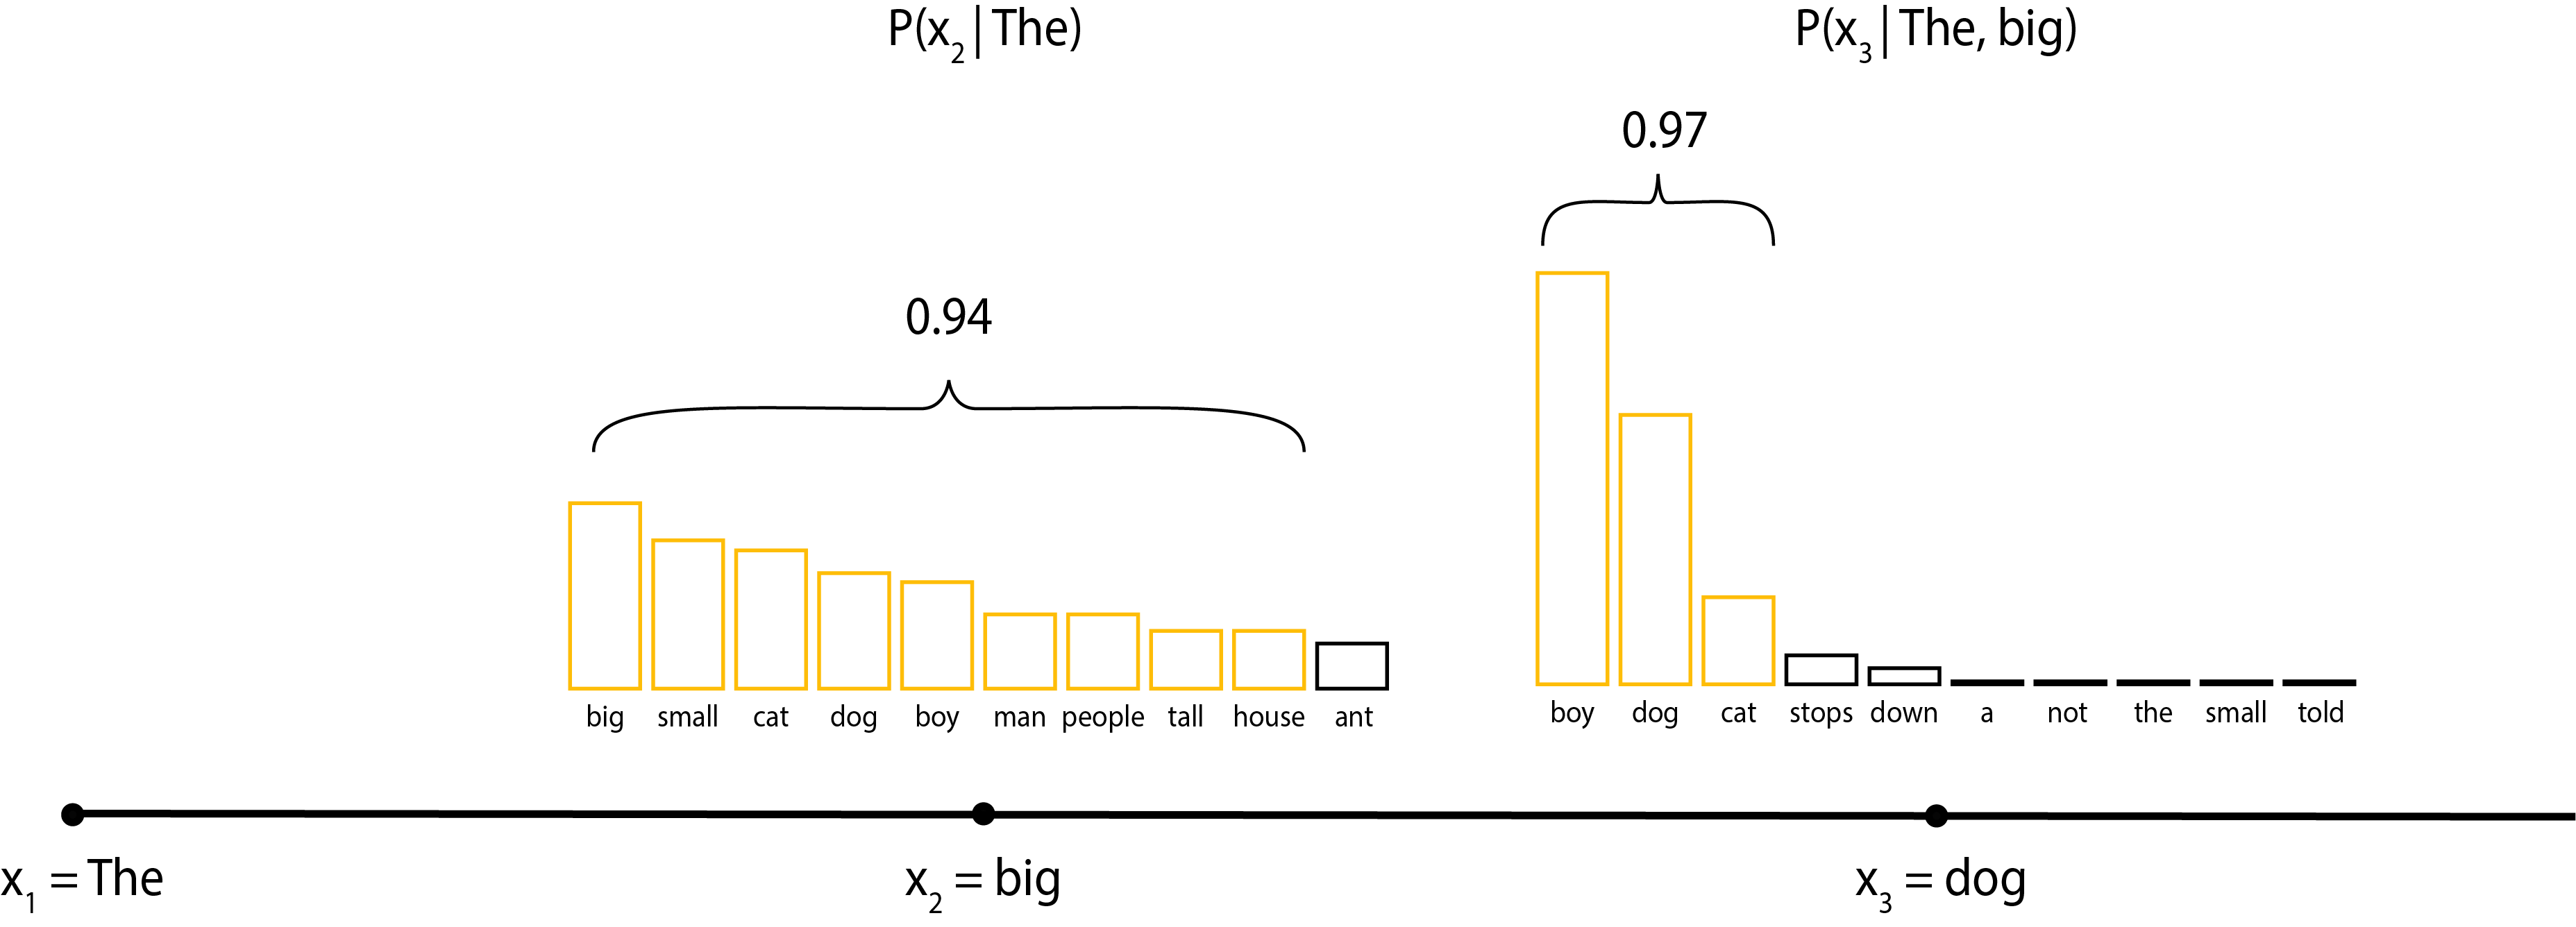
\includegraphics[width=0.9\columnwidth]{imgs/background/topp.png}
 \caption{Example top-p sampling for text generation with prior $x = [\textit{The}]$ \cite{platen2020}.}
 \label{fig:topp}
\end{figure}

The nucleus for $p=92\%$ includes the nine most likely words in the first step and only three words in the second step. This example highlights that top-p sampling keeps a wide range of tokens in less predictable situations (e.g. step $t=1$) and a few words when the next word seems more predictable (e.g. step $t=2$). Although top-p is theoretically more interesting than top-k, both methods work well in practice. Top-p can also be combined with top-k to avoid very low ranked words while allowing for some dynamic selection.

\subsection{Greedy Search}

Greedy search is the most basic decoding algorithm based on search. It consists of selecting the token with the highest probability at each generation step $t$: $x_t = argmax \, P(x_t|x_{1:t-1})$. Figure \ref{fig:greedy} shows a text generation example similar to the previous ones but with greedy decoding.
Starting with the prior sequence $x = [\textit{The}]$, in step $t=1$, the algorithm selects the word $\textit{nice}$ with has the highest probability among the three options $\{ \textit{dog}, \textit{nice}, \textit{car} \}$. In step $t=2$, the options are $\{ \textit{woman}, \textit{house}, \textit{guy} \}$ and the algorithm greedly selects \textit{woman}. Thus, the final generated sentence is \textit{The nice woman} with a joint probability of $0.5*0.4=0.2$.

\begin{figure}[!h]
 \centering
 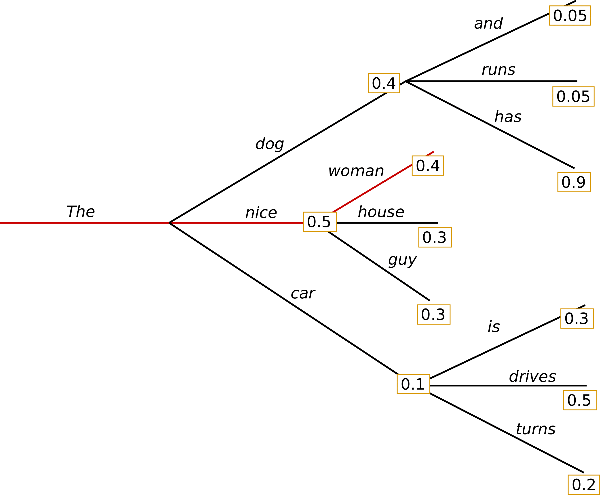
\includegraphics[width=0.7\columnwidth]{imgs/background/greedy.png}
 \caption{Example of greedy search for text generation with prior $x = [\textit{The}]$ \cite{platen2020}.}
 \label{fig:greedy}
\end{figure}

The problem with greedy search is that it misses high probability tokens ``hidden behind'' low probability ones. In this example, the global optimal solution is the sentence \textit{The dog has} (with joint probability $0.36$), but the word \textit{nice} has higher probability than \textit{dog} in step $t=1$. Thus, the greedy search selects \textit{nice} and completely disregards the branch with the word \textit{dog} in step $t=2$.

\subsection{Beam Search}

\textit{Beam search} reduces the risk of missing hidden high probability tokens by keeping the most likely $b$ solutions (called \textit{beams}) at each time step, where $b$ is a parameter called \textit{beam width}. At the final generation step, the solution (or beam) with the highest joint probability is selected. Figure \ref{fig:beam} shows how beam search is capable of finding the best solution of the previous example with beam size $b=2$. In step $t=1$, the two most likely sub-sequences are $\{ \textit{The}, \textit{dog} \}$ and $\{ \textit{The}, \textit{nice} \}$. In step $t=2$, beam search expands the beam from the previous step with the two most likely sub-sequences $\{ \textit{The}, \textit{dog}, \textit{has} \}$ and $\{ \textit{The}, \textit{nice}, \textit{woman} \}$. At the end of the second step, beam search returns the beam with highest probability which is \textit{The dog has} with joint probability $0.36$. The solutions generated with beam search are always as good as or better (more likely according to the LM) than the sequences generated with greedy search. However, beam search is not guaranteed to find the optimal sequence.

\begin{figure}[!h]
 \centering
 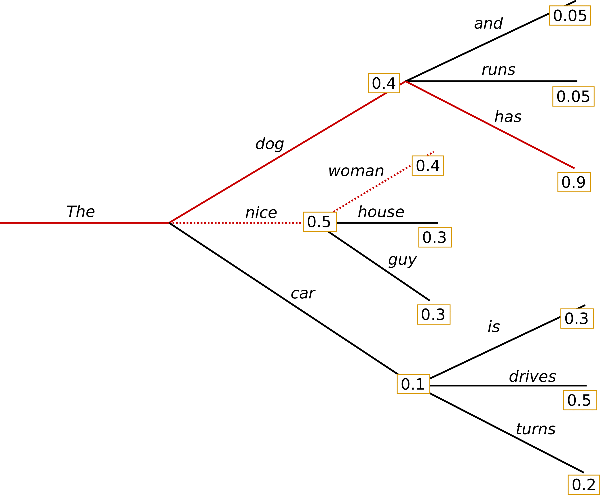
\includegraphics[width=0.7\columnwidth]{imgs/background/beam.png}
 \caption{Example of beam search for text generation with prior $x = [\textit{The}]$ and
 beam size $b=2$ \cite{platen2020}.}
 \label{fig:beam}
\end{figure}

A common problem of beam search decoding (and other search-based approaches) is that the decoded sequences present became repetitive in a few generation steps \cite{holtzman2019curious}. This problem can be aliviated by combining beam search with sampling (including top-k or top-p strategies) to create a \textit{Stochastic Beam Search} \cite{poole2010artificial}. In this case, the sub-sequences are sampled at each time step according to their joint probability, instead of selected greedly.

Different \textit{decoding} strategies (e.g. top-k sampling and beam search) can be used to generate music with different NN \textit{architectures} (e.g. LSTM, Transformer, VAEs, GANs) trained with different \textit{symbolic music} datasets (e.g. MAESTRO, Lakh, JSB Chorales). This chapter presented an overview
of these fundamental ideas of deep learning for music generation. This dissertation builds upon these ideas for controlling the perceived emotion of music composed by deep generative models. The next chapter discusses the previous related works with a similar goal of this dissertation: AMC systems that control perceived emotion, controllable LMs, and conditional generative models that control structural music features.
